%%%%%%%%%%%%%%%%%%%%%%%%%%%%%%%%%%%%%%%%%
% Masters/Doctoral Thesis 
% LaTeX Template
%%%%%%%%%%%%%%%%%%%%%%%%%%%%%%%%%%%%%%%%%

\documentclass[
11pt,
english,
singlespacing,
headsepline,
]{MastersDoctoralThesis}

\usepackage[utf8]{inputenc}
\usepackage[T1]{fontenc}

\usepackage{mathpazo}

\usepackage[numbers]{natbib}

\usepackage[autostyle=true]{csquotes}

\usepackage{booktabs}
\usepackage{float}
% Allows line breaks in long URLs, particularly in the bibliography.
\usepackage{xurl}
\Urlmuskip=0mu plus 1mu\relax

\geometry{
	paper=a4paper,
	inner=2.5cm,
	outer=3.8cm,
	bindingoffset=.5cm,
	top=1.5cm,
	bottom=1.5cm,
}

%----------------------------------------------------------------------------------------
%	THESIS INFORMATION
%----------------------------------------------------------------------------------------

\thesistitle{Digital Index of Territorial Adaptation Solutions to Population Ageing}
\supervisor{Marion \textsc{Scheider-Yilmaz}}
\examiner{}
\degree{Master 2 -- Natural Language Processing}
\author{Thomas \textsc{Francois}}
\addresses{}

\subject{Natural Language Processing}
\keywords{population ageing, natural language processing, information retrieval, textual data, digital humanities}
\university{\href{https://www.univ-lorraine.fr}{University of Lorraine}}
\department{}
\group{International Chair ``Inclusive Societies and Ageing'' -- SIAGE}
\faculty{}

\AtBeginDocument{
\hypersetup{
    pdftitle=\ttitle,
    pdfauthor=\authorname,
    pdfkeywords=\keywordnames,
    colorlinks=true,
    linkcolor=red,
    citecolor=red,
    urlcolor=red
}
}

\begin{document}

\frontmatter

\pagestyle{plain}

%----------------------------------------------------------------------------------------
%	TITLE PAGE
%----------------------------------------------------------------------------------------

\begin{titlepage}
\begin{center}

\vspace*{0.05\textheight}

\begin{minipage}[c]{0.44\textwidth}
    \centering
\includegraphics[width=0.72\linewidth]{Figures/Unuiversite-de-Lorraine_Logo.png}
\end{minipage}
\hfill
\begin{minipage}[c]{0.44\textwidth}
    \centering
\includegraphics[width=0.72\linewidth]{Figures/IDMC_Logo.png}
\end{minipage}

\vspace{1.4cm}

\textsc{\Large Internship Thesis}\\[0.5cm]

\HRule \\[0.4cm]
{\huge \bfseries \ttitle\par}\vspace{0.4cm}
\HRule \\[1.4cm]

\begin{minipage}[t]{0.4\textwidth}
\begin{flushleft} \large
\emph{Author:}\\
\authorname
\end{flushleft}
\end{minipage}
\begin{minipage}[t]{0.4\textwidth}
\begin{flushright} \large
\emph{Supervision:}\\
Academic supervisor: Maxime \textsc{Amblard}\\
Internship supervisor: Marion \textsc{Scheider-Yilmaz}
\end{flushright}
\end{minipage}\\[2.5cm]

\vfill

\large \textit{A thesis submitted as part of the requirements\\
for the degree of \degreename}\\[0.3cm]
\textit{in the}\\[0.4cm]
\groupname\\
\deptname\\[1.5cm]

\vfill

{\large Academic year 2025--2026}\par

\end{center}
\end{titlepage}

%----------------------------------------------------------------------------------------
%	DECLARATION PAGE
%----------------------------------------------------------------------------------------

\begin{declaration}
\addchaptertocentry{\authorshipname}
\noindent I, \authorname, declare that this thesis titled, \enquote{\ttitle}, and the work presented in it are my own. I confirm that:

\begin{itemize} 
\item This work was carried out during my internship within the International Chair ``Inclusive Societies and Ageing'' -- SIAGE.
\item Where I have consulted the published work of others, this is clearly attributed.
\item Where I have quoted from the work of others, the source is always given.
\item I have acknowledged all main sources of help.
\end{itemize}
 
\noindent Signed:\\
\rule[0.5em]{25em}{0.5pt}
 
\noindent Date:\\
\rule[0.5em]{25em}{0.5pt}
\end{declaration}

\cleardoublepage

%----------------------------------------------------------------------------------------
%	ABSTRACT PAGE
%----------------------------------------------------------------------------------------

\begin{abstract}
\addchaptertocentry{\abstractname}
Population ageing requires territorial responses in housing, mobility, health,
social participation, digital inclusion, and support for caregivers. Relevant
initiatives are documented by public institutions, associations, and local
authorities, but the resources are scattered across heterogeneous web pages,
PDF documents, and action sheets. This thesis presents \textit{Index\_Insight},
a reproducible pipeline that transforms this dispersed documentation into a
structured corpus for exploratory analysis.

The corpus contains 1,153 documents from six sources: CNAV, Fondation de
France, HCFEA, IReSP Autonomie, the SIAGE action-sheet corpus, and the
Francophone Age-Friendly Cities and Communities network (RFVAA). The pipeline
combines source-specific collection, text normalisation, relevance scoring,
structured extraction, and quality-control outputs. An initial rule-based
pipeline was progressively complemented by local LLM-assisted extraction using
Qwen2.5 through Ollama, with constrained JSON generation and controlled
metadata values.

The work delivers a documented corpus and analytical outputs describing themes,
initiative types, stakeholders, territories, and temporal information. The
evaluation distinguishes metadata completion from factual correctness: the
former is measured automatically, whereas the latter is assessed through human reference annotations. The thesis discusses the benefits and limitations of local
LLM-assisted extraction for heterogeneous territorial data, and identifies the
conditions required before the corpus can support a public search interface or
decision-support use.
\end{abstract}

%----------------------------------------------------------------------------------------
%	ACKNOWLEDGEMENTS
%----------------------------------------------------------------------------------------

\begin{acknowledgements}
\addchaptertocentry{\acknowledgementname}
I would like to thank my academic supervisor, Maxime Amblard, and my internship supervisor, Marion Scheider-Yilmaz, for their guidance and support throughout this internship. I also thank the SIAGE Chair and the INSIGHT project team for their feedback and for providing the scientific and interdisciplinary context of this work.
\end{acknowledgements}

%----------------------------------------------------------------------------------------
%	LIST OF CONTENTS/FIGURES/TABLES PAGES
%----------------------------------------------------------------------------------------

\tableofcontents

%\listoffigures
%\listoftables

%----------------------------------------------------------------------------------------
%	ABBREVIATIONS
%----------------------------------------------------------------------------------------

\begin{abbreviations}{ll}

\textbf{NLP} & \textbf{N}atural \textbf{L}anguage \textbf{P}rocessing\\
\textbf{IR} & \textbf{I}nformation \textbf{R}etrieval\\
\textbf{LLM} & \textbf{L}arge \textbf{L}anguage \textbf{M}odel\\
\textbf{JSON} & \textbf{J}ava\textbf{S}cript \textbf{O}bject \textbf{N}otation\\
\textbf{SIAGE} & \textbf{S}ociétés \textbf{I}nclusives et \textbf{A}vancée en \textbf{A}ge\\
\textbf{INSIGHT} & Research project related to territorial adaptation and ageing\\
\textbf{API} & Application Programming Interface\\
\textbf{BERT} & Bidirectional Encoder Representations from Transformers\\
\textbf{BM25} & Best Matching 25\\
\textbf{CNAV} & Caisse nationale de l'assurance vieillesse\\
\textbf{CSV} & Comma-Separated Values\\
\textbf{EHPAD} & Établissement d'hébergement pour personnes âgées dépendantes\\
\textbf{HCFEA} & Haut Conseil de la famille, de l'enfance et de l'âge\\
\textbf{HTML} & HyperText Markup Language\\
\textbf{HTTP} & HyperText Transfer Protocol\\
\textbf{IReSP} & Institut de recherche en santé publique\\
\textbf{PDF} & Portable Document Format\\
\textbf{TF--IDF} & Term Frequency--Inverse Document Frequency\\
\textbf{RFVAA} & Réseau francophone des Villes Amies des Aînés\\

\end{abbreviations}

%----------------------------------------------------------------------------------------
%	DEDICATION
%----------------------------------------------------------------------------------------

% No dedication page in this version.
% \dedicatory{}

%----------------------------------------------------------------------------------------
%	THESIS CONTENT - CHAPTERS
%----------------------------------------------------------------------------------------

\mainmatter

\pagestyle{thesis}

\chapter{Introduction}

\section{Internship context}

Population ageing raises interconnected challenges for housing, mobility, access
to healthcare, social participation, digital inclusion, and support for caregivers.
These challenges are addressed not only through national policy frameworks, but
also through locally designed initiatives carried by municipalities, associations,
social-protection organisations, care providers, and citizen groups. Such
initiatives constitute situated forms of knowledge: they document how actors in a
specific territory identify local needs and develop responses to them.

This internship was carried out within the International Chair ``Inclusive
Societies and Ageing'' (SIAGE) at the University of Lorraine and contributes to
the INSIGHT research project. SIAGE brings together research in the social
sciences, public-policy studies, and technical disciplines in order to examine the
conditions of inclusion and exclusion associated with ageing. Its work is concerned
with both the diversity of older adults' life courses and the role of social,
institutional, physical, and digital environments in supporting participation,
autonomy, and citizenship.

Among its participatory action-research activities, the Chair develops the
\textit{Senior Citizen Design Workshops}. Developed in France since 2018 in
collaboration with local authorities and the international REIACTIS network, this
approach aims to involve older adults as citizens rather than only as users or
beneficiaries of public action. The workshops are organised around four connected
stages: participatory diagnosis, citizen-centred co-design, dialogue with public
decision-makers, and follow-up and evaluation. They produce action sheets and
other textual material in which participants describe local problems, proposed
solutions, actors, and territorial resources.

The documentary material available to the project extends beyond the action sheets
produced within the Senior Citizen Design Workshops. Numerous initiatives are also
carried locally by other territorial and gerontological actors. Their websites,
reports, project descriptions, and practical sheets contain valuable, localised
knowledge about responses to ageing-related challenges. However, this knowledge is
dispersed across organisations, territories, formats, and editorial practices.

Taken together, these resources form a large but heterogeneous French-language
corpus. They are partially structured and difficult to mobilise systematically for
researchers, local practitioners, policy-makers, and older citizens who may wish
to identify or draw inspiration from initiatives developed in other territories.
The purpose of \textit{Index\_Insight} is to make this dispersed material more
visible, comparable, and reusable while preserving its documentary provenance.

\section{Problem statement}

Although the corpus contains rich descriptions of local responses to population
ageing, the absence of a shared structure limits its practical and scientific use.
It is difficult to search across territories, compare initiative types, identify the
actors involved, or examine the themes and needs addressed by the documented
initiatives. This scarcity of accessible and comparable information limits the
capacity of researchers to analyse local ageing policies, of practitioners and local
elected representatives to identify transferable experiences, and of older citizens
to learn from initiatives developed elsewhere.

This is also a natural language processing problem. The documents do not use a
common template: a target audience, territorial scale, initiative holder, or date
may appear in a heading, a table, a paragraph, or not be stated at all. Relevant
information can be expressed through varied French formulations, while PDF
extraction and web scraping may introduce boilerplate, broken encoding, or missing
layout information. A useful system must therefore do more than fill database
fields: it must distinguish absent information from extraction failure, retain a
link to the source, and make uncertain outputs reviewable.

The problem addressed in this internship is consequently not only the technical
extraction of information from text. It is the design of a documented and
interdisciplinary workflow capable of transforming heterogeneous documentary
resources into structured metadata that can support exploration, comparison,
capitalisation of experience, and the circulation of knowledge between territories.
The intended result is an exploratory index, rather than an exhaustive inventory
of initiatives or a system that evaluates their quality or effectiveness.

\section{Objectives of the thesis}

The objective of this work is to design and implement a prototype tool based on
natural language processing techniques. More specifically, the project aims to:

\begin{enumerate}
    \item collect French-language documentary resources from multiple sources and
    preserve their raw content and provenance;
    \item clean and organise these heterogeneous materials into a coherent,
    traceable corpus;
    \item extract structured metadata relevant to the description of territorial
    initiatives, using both rule-based methods and a constrained local language
    model;
    \item normalise selected themes and initiative types into controlled French
    vocabularies while retaining the original extracted labels; and
    \item evaluate the observed quality of selected metadata fields against human
    annotations, and identify the limits of the resulting descriptive analyses.
\end{enumerate}

\paragraph{Research question.}
This internship addresses the following research question: \emph{to what extent
can a locally deployed language model transform heterogeneous textual
descriptions of territorial initiatives related to population ageing into
reliable, structured, and reusable metadata?} Three operational questions
follow: (i) how can documents with different formats and editorial structures be
collected and normalised in a traceable way; (ii) which metadata can be extracted
under controlled vocabularies; and (iii) how should corpus quality be assessed
without confusing field completion with factual correctness?

\section{Scope of the prototype}

\textit{Index\_Insight} focuses on French-language textual resources that describe
initiatives, projects, services, or reflections related to ageing and territorial
inclusion. Its structured records are intended to support documentary retrieval and
exploratory comparison. They do not constitute an evaluation of an initiative's
impact, a ranking of territories, or a representation of all initiatives existing
in France. The system is likewise not designed to make decisions about people or
organisations. These boundaries are important because the corpus reflects the
availability and editorial choices of its sources as much as it reflects the
underlying initiatives.

\section{Contributions}

The first contribution of this internship is a documented corpus of 1,153
resources from six complementary sources. The collection is accompanied by a data
architecture that separates raw documents, intermediate processing artefacts,
structured outputs, and evaluation material. This organisation makes it possible
to inspect each stage of the workflow and to revisit a record when a source or an
extraction decision needs to be checked.

The second contribution is an extraction pipeline adapted to documentary
heterogeneity. It combines a transparent rule-based baseline with a local LLM
workflow that uses a French prompt, controlled labels, and machine-readable JSON
outputs. The pipeline produces metadata covering target audience, initiative type,
theme, territorial scale, territory, initiative holder, and date. A deterministic
normalisation layer then improves comparability between documents without
overwriting the original model outputs.

The third contribution is an initial empirical evaluation of the LLM-assisted
metadata. A human-annotated, source-stratified sample makes it possible to report
field-level quality rather than relying solely on output completeness. Together
with provenance fields and archived raw responses, this evaluation positions the
prototype as a reviewable research tool and provides concrete priorities for
future improvement, especially for temporally ambiguous information.

\section{Structure of the thesis}

Chapter~2 reviews related work on information extraction, named entity
recognition, text classification, large language models, and information
retrieval. Chapter~3 presents the corpus, the collection process, the data model,
and the extraction methodology. Chapter~4 describes the implementation and the
reproducibility measures adopted in the project. Chapter~5 reports the evaluation
protocol and results. Chapter~6 discusses the contributions, limitations, ethical
considerations, and possible uses of the index. Finally, Chapter~7 summarises the
work and outlines the main directions for future development.


\chapter{General Context of the Project}

\section{Host institution and research setting}

This internship was carried out within the International Chair ``Inclusive
Societies and Ageing'' (SIAGE) at the University of Lorraine. The Chair studies
population ageing through the question of inclusive societies: how can social,
institutional, physical, and digital environments support the participation,
autonomy, rights, and citizenship of older adults? This perspective does not
reduce ageing to an individual health issue. It also considers life courses,
social inequalities, public policies, professional practices, and territorial
configurations that can facilitate or hinder inclusion.

SIAGE develops an interdisciplinary research environment that brings together
social sciences, public-policy studies, public health, engineering, and digital
technologies. Its objective is to connect academic research with territorial
actors, public decision-makers, professionals, associations, and older citizens.
Within this setting, digital methods are useful when they help organise and
compare dispersed knowledge, but their interpretation remains dependent on the
social and territorial context in which initiatives are developed.

The internship also contributes to the INSIGHT project. INSIGHT promotes the
connection of Natural Language Processing and Artificial Intelligence with
research in the Humanities and Social Sciences. \textit{Index\_Insight} is a
concrete application of this orientation: it uses NLP methods to make a large
and heterogeneous body of documentation on territorial adaptation to ageing more
accessible for research and future operational use.

\section{Senior Citizen Design and territorial knowledge}

One of the SIAGE Chair's participatory action-research activities is the
\textit{Senior Citizen Design} approach. Developed in France since 2018 in
collaboration with local authorities and the REIACTIS network, it seeks to
involve older adults as citizens rather than only as users or beneficiaries of
public action. The approach is structured around four connected stages:
participatory diagnosis, citizen-centred co-design, dialogue with public
decision-makers, and follow-up and evaluation.

The Senior Citizen Design Workshops produce action sheets in which participants
describe local issues, proposed responses, target publics, actors, and resources.
These documents are valuable because they preserve knowledge produced through
participatory work. However, they represent only one part of the relevant
documentary landscape. Numerous other initiatives are carried by municipalities,
associations, social-protection organisations, care providers, and networks
specialised in ageing. Their websites, reports, project descriptions, and
practical sheets also document locally situated responses to ageing-related
challenges.

\section{The role of Index\_Insight}

The aim of \textit{Index\_Insight} is not simply to create a collection of
documents. It is to capitalise territorial initiatives, make them visible and
comparable, and facilitate the circulation of experience between territories. A
structured index can support several uses: researchers can explore how local
ageing-related issues are described; territorial actors can identify relevant
examples; and participants in Senior Citizen Design Workshops can draw on
initiatives developed elsewhere when discussing local needs and possible
responses.

This objective creates a specific NLP problem. The relevant information is not
held in a homogeneous database: it is dispersed across sources with different
formats, vocabularies, levels of detail, and editorial structures. Titles,
territories, target audiences, initiative holders, dates, themes, and descriptions
may be explicit, implicit, absent, or located in different parts of a source
document. The task is therefore to transform these heterogeneous resources into
structured, traceable metadata without erasing their provenance or presenting
automatic inferences as established facts.

The design of the Index was informed by dialogue between its technical development
and the SIAGE research team. This dialogue contributes to the selection of sources,
the definition of metadata fields, the vocabulary used for quality control, and the
interpretation of the outputs. It is essential because the technical schema must
remain useful for the concrete questions addressed in participatory diagnosis,
co-design, dialogue with decision-makers, and the capitalisation of experience.

\section{Corpus, stakeholders, and constraints}

The corpus combines two complementary forms of documentation. The first consists
of action sheets produced by older adults themselves within Senior Citizen Design
Workshops implemented by SIAGE. The second consists of initiative descriptions
published by institutional, associative, and territorial actors involved in the
adaptation of territories to population ageing in France. The external sources were
selected in dialogue with the SIAGE team according to their relevance to the scope
of the Index and the availability of sufficiently substantial material for
structuring.

The intended users are correspondingly diverse: researchers studying ageing and
local public action, SIAGE participants and facilitators, local elected
representatives and practitioners, associations, and, in the longer term, older
citizens. Their needs are not limited to finding a document. They include comparing
initiative types, identifying territorial scales and stakeholders, locating examples
related to a particular issue, and understanding the limits of the available
documentation.

The main technical constraints arise from the organisation of the field itself.
The French gerontological landscape includes actors operating at national,
regional, departmental, intermunicipal, and local levels, with complementary
objectives in prevention, housing, mobility, health, participation, digital
inclusion, and social connection. This multi-level governance produces a naturally
fragmented documentary landscape. Relevant information may be distributed across
several pages of the same website, embedded in PDF documents, or expressed through
source-specific terminology. The collection, normalisation, and structured
extraction pipeline described in the following chapters is a response to this
documentary and institutional heterogeneity.


\chapter{State of the Art}

\section{Information Retrieval and Document Indexing}

The increasing availability of digital textual resources has made information retrieval (IR) a central field in computer science and natural language processing. Information retrieval systems aim to organize, index, and retrieve relevant information from large collections of documents. In the context of this project, IR methods are particularly relevant because the corpus consists of heterogeneous textual documents collected from multiple institutional and associative sources.

Document indexing refers to the process of transforming raw documents into structured representations that can be efficiently searched and analysed. One of the most influential weighting methods is TF-IDF (\textit{Term Frequency -- Inverse Document Frequency}), introduced by Salton and Buckley \citep{salton1988term}. TF-IDF assigns higher importance to terms that frequently appear in a document while remaining relatively rare across the corpus. This allows systems to identify terms that are more discriminative for a given document.

More recent retrieval systems often rely on probabilistic ranking models such as BM25 \citep{robertson2009probabilistic}. BM25 improves document ranking by taking into account both term frequency and document length, making it particularly effective for heterogeneous corpora. Such approaches remain widely used in modern search engines and document retrieval systems because of their efficiency and interpretability.

Traditional information retrieval approaches mainly rely on exact lexical matching between queries and documents. However, these methods may struggle when semantically similar documents use different vocabulary. For example, documents referring to “older adults”, “senior citizens”, or “ageing populations” may discuss similar concepts while using different terms. This limitation has motivated the development of semantic search approaches.

Semantic retrieval methods use vector representations of words, sentences, or documents in order to capture semantic similarity rather than exact lexical overlap. Early approaches relied on word embeddings such as Word2Vec \citep{mikolov2013efficient}. More recent transformer-based models such as BERT \citep{devlin2019bert} significantly improved contextual text representations and semantic retrieval performance.

In addition to textual content, document indexing systems often rely on metadata. Metadata correspond to structured information associated with documents, such as titles, dates, authors, institutions, locations, or thematic categories. Metadata play a crucial role in document exploration because they enable filtering, faceted search, and corpus organization. In the context of territorial adaptation initiatives, metadata can include geographical information, target populations, types of stakeholders, or thematic domains such as mobility, housing, or social inclusion.

Another important aspect of document indexing concerns corpus heterogeneity. Documents collected from institutional websites, reports, PDF files, and action sheets often differ considerably in structure, formatting, vocabulary, and quality. Such heterogeneity complicates indexing and retrieval because information may be inconsistently represented across sources. As a result, preprocessing and normalization stages are essential before indexing can be performed effectively.

Recent developments in neural information retrieval combine classical indexing techniques with deep learning approaches. Dense retrieval methods represent documents as semantic embeddings that can be queried using similarity measures \citep{karpukhin2020dense}. These approaches are particularly useful for exploratory search and thematic analysis in large unstructured corpora.

In the context of this thesis, information retrieval and document indexing methods provide the theoretical foundations for organizing and exploring a heterogeneous corpus of territorial initiatives related to population ageing. The project therefore combines classical preprocessing and indexing approaches with more recent NLP-based methods to facilitate document exploration, comparison, and knowledge extraction.

\section{Data extraction and structuring}

Data extraction and structuring are essential components of modern information systems, particularly when dealing with heterogeneous and unstructured textual corpora. In many domains, including digital humanities, social sciences, and institutional documentation, relevant information is often distributed across web pages, reports, PDF files, or semi-structured documents. Extracting and organizing this information into structured representations is therefore a major challenge.

Traditional information extraction approaches generally rely on rule-based systems, pattern matching, or manually designed heuristics. These methods often use regular expressions, predefined templates, or linguistic rules to identify specific entities or information categories within texts. Rule-based extraction systems may perform well in constrained environments where documents follow highly regular structures. However, they tend to struggle when applied to heterogeneous corpora containing variable formatting, inconsistent writing styles, or incomplete information.

Several studies have highlighted the limitations of rule-based extraction methods for large-scale and heterogeneous textual datasets. According to \citet{grishman2019information}, handcrafted extraction pipelines require substantial manual effort and often lack robustness when documents originate from multiple sources with differing structures. Similarly, \citet{sarawagi2008information} note that information extraction becomes increasingly difficult when dealing with noisy, partially structured, or domain-specific documents.

Web data extraction presents additional challenges. Websites frequently use different HTML structures, dynamic content generation, or inconsistent metadata organization. As explained by \citet{mitchell2018web}, web scraping pipelines often require source-specific extraction strategies because the organization of textual content varies significantly across websites. PDF documents introduce further complexity because they are designed for visual rendering rather than semantic structure preservation. Text extraction from PDFs may therefore produce noisy outputs containing formatting artefacts, fragmented sentences, or inconsistent line breaks.

In order to address these issues, preprocessing and structuring operations are generally required before analysis can be performed. Typical preprocessing steps include text normalization, lowercasing, accent removal, punctuation cleaning, whitespace normalization, and segmentation. These operations help reduce superficial variability within the corpus and improve the consistency of downstream processing tasks.

Beyond simple text cleaning, document structuring aims to transform unstructured textual content into organized and searchable representations. Structured representations usually rely on metadata schemas describing documents according to predefined categories such as title, date, author, thematic domain, or geographical information. Metadata play a central role in corpus organization because they enable indexing, filtering, retrieval, and comparative analysis.

Controlled vocabularies and taxonomies are commonly used to improve metadata consistency. According to \citet{hedden2016taxonomy}, controlled vocabularies reduce ambiguity by restricting metadata fields to predefined categories or authorised terms. Such approaches are widely used in information science, digital libraries, and documentary indexing systems. They facilitate corpus exploration by ensuring that similar concepts are represented consistently across documents.

More recently, natural language processing and machine learning approaches have significantly transformed information extraction methods. Traditional extraction systems based on manually designed rules are progressively being complemented or replaced by statistical and neural approaches capable of adapting to more variable textual data.

Large language models (LLMs) have introduced new possibilities for structured information extraction. Transformer-based architectures such as GPT \citep{brown2020language} or Qwen are capable of performing extraction tasks through prompt engineering rather than explicit programming rules. Prompt-based extraction consists in instructing the model to generate structured outputs, often in formats such as JSON, based on natural language instructions and constraints.

Recent studies have shown that LLMs can produce competitive results for information extraction tasks, particularly in contexts involving heterogeneous or partially structured documents. According to \citet{wei2022chain}, prompt engineering allows language models to perform complex reasoning and structured generation tasks with limited task-specific training. Similarly, \citet{liu2023pre} highlight the growing importance of prompting strategies for controlling model outputs and improving consistency.

One important aspect of LLM-assisted extraction concerns constrained generation. In many applications, the objective is not only to extract information, but also to ensure that outputs follow a stable and machine-readable structure. JSON-based extraction has therefore become increasingly common because it facilitates downstream indexing, database integration, and search functionalities. Controlled prompts can impose structural constraints, semantic constraints, and predefined categories in order to reduce hallucinations and improve consistency.

However, LLM-based extraction also introduces new limitations. Outputs may contain hallucinated information, inconsistent formatting, ambiguous interpretations, or unstable category assignments. As noted by \citet{bommasani2021opportunities}, large language models remain probabilistic systems whose outputs depend strongly on prompt design and contextual information. Consequently, human verification often remains necessary, especially in scientific or institutional contexts.

In the context of this thesis, data extraction and structuring methods provide the theoretical foundations for transforming heterogeneous textual resources related to territorial adaptation to ageing into a structured and searchable corpus. The project therefore combines traditional preprocessing methods, controlled vocabularies, and prompt-guided LLM extraction in order to produce coherent structured representations from heterogeneous institutional documents.


Data extraction involves collecting textual information from sources such as web pages or PDF documents. Structuring this data is essential for analysis.

\section{Natural language processing}

Natural language processing (NLP) refers to a set of computational methods designed to analyse, process, and generate human language. NLP combines approaches from computer science, linguistics, artificial intelligence, and statistics in order to enable automatic processing of textual data. In the context of this project, NLP methods play a central role because the corpus consists entirely of unstructured or semi-structured textual resources related to territorial adaptation and population ageing.

Traditional NLP pipelines generally rely on several preprocessing stages. One of the most fundamental operations is tokenisation, which consists in splitting a text into smaller units such as words, punctuation marks, or sentences. Tokenisation provides the basis for most downstream processing tasks because it transforms raw text into analysable units. Sentence segmentation is also important in order to identify discourse boundaries and improve text organization.

Another important preprocessing operation is text normalisation, which aims to reduce superficial textual variability through transformations such as lowercasing, accent removal, punctuation cleaning, and whitespace standardisation. According to \citet{manning1999foundations}, such preprocessing operations improve corpus consistency and facilitate indexing and retrieval tasks. In multilingual or heterogeneous corpora, normalization also helps reduce noise introduced by formatting differences or inconsistent orthography.

Lemmatization and stemming are commonly used techniques for reducing inflected words to more canonical forms. Stemming methods generally remove suffixes in order to approximate root forms, while lemmatization relies on linguistic analysis to recover dictionary forms. These approaches help reduce vocabulary sparsity and improve thematic grouping of semantically related terms.

Beyond preprocessing, NLP also includes methods for representing textual data computationally. Early approaches relied on sparse vector representations such as bag-of-words or TF-IDF. While effective for lexical matching, these methods often fail to capture semantic similarity between words or documents.

The development of distributed word representations significantly transformed NLP. Word embedding models such as Word2Vec \citep{mikolov2013efficient} represent words as dense vectors learned from large corpora. These representations capture semantic and syntactic relationships between words by placing semantically similar terms close together in vector space.

More recently, transformer-based architectures have become dominant in NLP. Transformers were introduced by \citet{vaswani2017attention} and rely on self-attention mechanisms capable of modelling contextual relationships between words. Unlike previous sequential architectures, transformers can process entire sequences simultaneously, which greatly improves scalability and contextual representation.

One of the most influential transformer-based models is BERT (\textit{Bidirectional Encoder Representations from Transformers}) proposed by \citet{devlin2019bert}. BERT introduced bidirectional contextual embeddings, allowing words to be interpreted according to both left and right contexts. This significantly improved performance on many NLP tasks such as classification, named entity recognition, question answering, and semantic similarity.

The emergence of large language models (LLMs) further expanded the capabilities of NLP systems. Models such as GPT \citep{brown2020language} or Qwen are trained on massive textual corpora and are capable of performing a wide range of tasks through prompting rather than task-specific programming. These models can generate text, summarise documents, classify information, answer questions, and extract structured information from unstructured inputs.

Prompt engineering has therefore become an important aspect of modern NLP workflows. Prompt engineering consists in designing textual instructions that guide model behaviour and constrain outputs. According to \citet{liu2023pre}, prompting strategies play a crucial role in controlling the quality, consistency, and reliability of LLM outputs. Prompt design may include formatting instructions, controlled vocabularies, examples, or explicit reasoning constraints.

In addition to text generation, NLP methods are increasingly used for information extraction and document structuring. Named entity recognition (NER), topic modelling, semantic similarity analysis, and text classification are commonly applied to large documentary corpora. In social sciences and digital humanities, these approaches facilitate the exploration of large collections of textual resources that would otherwise be difficult to analyse manually.

The use of NLP in institutional and social-science-related corpora nevertheless presents several challenges. Documents are often heterogeneous, partially structured, and domain-specific. Vocabulary may vary between institutions, and important information may be implicit rather than explicitly stated. As a result, purely rule-based methods frequently struggle to generalize across datasets.

Recent work therefore increasingly combines traditional preprocessing techniques with transformer-based or LLM-based approaches capable of contextual interpretation. Such models are particularly useful when information extraction requires semantic understanding rather than simple keyword matching.

In the context of this thesis, NLP methods provide the theoretical and technical foundations for transforming heterogeneous textual resources into structured and searchable representations. The project combines preprocessing techniques, controlled vocabularies, prompt engineering, and LLM-assisted extraction in order to facilitate indexing, comparison, and exploration of territorial initiatives related to population ageing.


\section{Comparable systems}

Several families of systems address parts of the problem considered in this
thesis, although few combine all of its requirements: heterogeneous French
source material, traceable collection, controlled metadata, and exploratory
analysis of territorial initiatives.

A first family consists of documentary catalogues and digital-library systems.
They organise resources through bibliographic or descriptive metadata and
provide faceted browsing by author, date, subject, institution, or place. Their
main strength is the use of stable metadata schemas and controlled vocabularies,
which improve consistency and make filtering possible. As noted in work on
taxonomies and controlled vocabularies, this standardisation reduces ambiguity
and supports reliable indexing \citep{hedden2016taxonomy}. However, catalogue
systems usually assume that metadata are supplied by publishers or cataloguers.
They do not by themselves solve the extraction of structured information from
long, heterogeneous web pages, reports, and action sheets.

A second family consists of search and information-retrieval systems. Lexical
engines based on inverted indexes, TF--IDF, or BM25 can efficiently retrieve
documents that contain query terms \citep{salton1988term,robertson2009probabilistic}.
They are well suited to transparent keyword search and can be combined with
facets based on manually supplied metadata. Dense retrieval extends this
approach by representing queries and documents in a shared semantic vector
space \citep{karpukhin2020dense}. Such systems are useful when users express a
need with words that differ from those used in the source documents. Their
limitation for the present project is that retrieval alone does not create the
territorial, organisational, temporal, and thematic metadata required for
comparative analysis.

A third family is constituted by rule-based information-extraction pipelines.
These pipelines use document templates, headings, regular expressions,
lexicons, and pattern-matching rules to identify candidate values. They are
particularly appropriate when source structures are stable because their
decisions can be inspected and corrected. Their limitations have been widely
documented: rules require substantial maintenance and generalise poorly when
documents come from sources with different editorial structures
\citep{sarawagi2008information,grishman2019information}. This limitation is
central in the present corpus, which contains HTML pages, PDF-derived text, and
internally produced action sheets.

More recent systems use transformer-based language models to classify,
summarise, or extract information from text. Prompt-guided LLM extraction makes
it possible to request a predefined JSON schema directly from a document, while
the prompt can specify controlled values and rules for unknown information.
This approach benefits from the contextual modelling capabilities of
transformers \citep{vaswani2017attention,devlin2019bert} and from the flexible
task formulation enabled by large language models \citep{brown2020language}.
It also introduces important risks: a generated field can be fluent and
complete while remaining unsupported by the source. Prompting strategies,
output constraints, and explicit validation are therefore necessary
\citep{liu2023pre}.

The project is not intended to replace a mature public search platform or a
digital library. Rather, it occupies an intermediate position between a
collection pipeline and a future exploration system. Its immediate contribution
is to transform dispersed documentary material into traceable JSON records that
can subsequently support catalogue-like filtering, lexical search, descriptive
statistics, and, in later work, semantic or hybrid retrieval.

\begin{table}[H]
\centering
\begin{tabular}{p{3.2cm}p{3.5cm}p{3.5cm}p{3.4cm}}
\toprule
Approach & Main strength & Main limitation for this corpus & Position of Index\_Insight \\
\midrule
Documentary catalogue & Stable metadata and faceted navigation & Assumes metadata already exist or are manually curated & Reuses the principle of controlled metadata, but automates part of their production \\

Lexical or dense retrieval & Efficient retrieval and exploration of large collections & Does not itself extract reliable documentary metadata & Future use of the structured corpus; not yet a deployed search engine \\

Rule-based extraction & Transparent and inspectable decisions & Fragile across heterogeneous document structures & Baseline and quality-control layer of the pipeline \\

LLM-assisted extraction & Context-sensitive structuring of varied documents & Risk of unsupported inference and output inconsistency & Constrained local extraction, evaluated against human reference annotations \\
\bottomrule
\end{tabular}
\caption{Positioning of Index\_Insight relative to comparable system families.}
\label{tab:comparable-systems}
\end{table}

\section{Synthesis of the state of the art}

The literature shows that no single technique is sufficient for organising a
heterogeneous documentary corpus. Classical information retrieval provides
efficient indexing and transparent lexical search, while dense retrieval can
later improve access to semantically related initiatives. Controlled
vocabularies provide the consistency required for filtering and comparison.
Rule-based extraction remains valuable for traceability and for inspecting
intermediate candidate values, but it becomes difficult to maintain when the
same information is expressed through different layouts and writing styles.
LLMs can reduce this dependence on source-specific rules by interpreting
context, provided that their outputs are constrained and independently checked.

These findings motivate the hybrid design adopted in this thesis. The pipeline
preserves raw sources and intermediate rule-based outputs, then uses a local
LLM to create structured records under a predefined JSON schema and controlled
metadata values. The local deployment supports reproducibility, cost control,
and data governance, while the retained provenance makes it possible to trace a
metadata value back to its source document. Crucially, the system does not treat
model output as self-validating. Completion rates measure technical coverage;
human reference annotation was used to assess factual correctness.

The contribution of \textit{Index\_Insight} is therefore not a claim that an
LLM alone can objectively describe territorial initiatives. It is the design of
a documented workflow that makes a dispersed corpus searchable and comparable,
while preserving the distinction between automatically generated metadata and
validated information. This position also defines the next stage of the
project: after corpus structuring and factual evaluation, the records can be
used to design a faceted, lexical, semantic, or hybrid exploration interface
with the future users of the INSIGHT project.

\chapter{Methodology}

\section{Overview of the approach}

The methodology follows a complete document-processing pipeline designed to
transform heterogeneous textual resources into a structured corpus that can
support search, filtering, comparison, and thematic analysis. The overall
objective is to make dispersed descriptions of territorial initiatives related
to population ageing more accessible for research and future operational use.

The methodological process evolved during the internship. The initial approach
relied on a multi-step rule-based pipeline: documents were cleaned, segmented,
analysed for document sections, and processed to extract candidate metadata
values. Candidate values were then scored according to explicit rules. This
approach was transparent and useful for inspecting intermediate results, but the
diversity of source formats and writing styles made it difficult to generalise
the extraction rules to every document type.

The final approach therefore complements this rule-based pipeline with
LLM-assisted information extraction. A local language model receives a
constrained prompt and transforms each textual document into a structured JSON
record. The methodology is consequently organised around seven components:
collection, corpus construction, cleaning and quality control, progressive
structuring, constrained LLM extraction, post-extraction taxonomy
normalisation, and evaluation.

\begin{figure}[H]
    \centering
    
\includegraphics[width=0.82\textwidth]{Figures/index-insight-pipeline.pdf}
    \caption{Architecture of the Index\_Insight pipeline. Heterogeneous
    documentary sources are collected and normalised before being processed by
    a traceable rule-based baseline and by constrained local LLM extraction.
    Structured records are evaluated against a human reference sample and used
    to generate exploratory analytical outputs.}
    \label{fig:index-insight-pipeline}
\end{figure}

\section{Data collection}

Data were collected from multiple sources using dedicated Python scripts. The
collection process focused on web pages, PDF documents, action sheets, and
project descriptions related to ageing, autonomy, social inclusion, housing,
mobility, health, participation, and support for caregivers. Each retained
resource was stored as a separate \texttt{.txt} file, following the principle
of one documentary record per file.

The corpus contains 1,153 textual documents. Sixty documents were provided
directly by the SIAGE Chair as action sheets, while the remaining documents were
collected from external institutional or associative sources. The collection
scripts use HTTP requests and HTML parsing to retrieve the textual content of
web pages. Additional processing is used when a relevant resource is provided
as a PDF document. Since the websites differ in navigation, HTML structure, and
metadata availability, the collection process relies on source-specific
strategies rather than on a single generic scraper.

The final cleaned corpus contains 1,153 documents and 917,554 word tokens,
corresponding to an average of 795.8 words per document. Document length ranges
from 8 to 3,573 words, illustrating the heterogeneous nature of the collected
material. The corpus is therefore composed primarily of medium-length resources
that usually contain sufficient contextual information to support extraction,
while still requiring robust processing because relevant information may occur
at different locations and be expressed in highly variable forms.

The collection process preserves a link between each record and its source.
This provenance is necessary for quality control, source attribution, correction
of extraction errors, and future updates. The project is intended for
documentary and exploratory purposes; collection should therefore continue to
respect the terms of access of the relevant websites and avoid excessive request
rates.

For every LLM-generated record, the final index also stores explicit provenance
metadata: \texttt{source\_site}, \texttt{source\_url},
\texttt{original\_title}, and \texttt{collection\_date}. These fields are
populated deterministically from the collection indexes and archived source
files; they are not generated by the language model. The source URL points to
the original web page or PDF when it is available, whereas the internal SIAGE
action sheets are identified as such and do not receive an artificial public
URL. The original title preserves the wording supplied by the source and makes
it possible to distinguish the source document from a normalised or extracted
metadata value.

At the time of analysis, all 1,143 available LLM records contained a
standardised source identifier. A source URL was available for 1,083 external
records; the remaining 60 records correspond to SIAGE internal action sheets.
An original title was available for 1,142 records, with one RFVAA record lacking
a title in its source index. These coverage figures make missing provenance
visible rather than replacing it with generated or inferred information.

The historical collection indexes did not consistently record a reliable
collection timestamp. The \texttt{collection\_date} field is therefore left
empty for these legacy records rather than being reconstructed from file-system
dates, which would be misleading. Future collection scripts should record the
timestamp automatically at download time, using an ISO 8601 date. Together,
these provenance fields support attribution, verification against the original
document, correction of metadata, and responsible reuse of externally collected
materials.

\section{Corpus construction}

The corpus was built from two complementary types of material. First, the SIAGE
Chair provided internal action sheets collected in the context of previous work
on territorial adaptation to population ageing. Second, external institutional
and associative websites were selected because they contained practical sheets,
initiative descriptions, research-project records, or public-action resources
related to the project's scope.

Only documents containing a sufficiently substantial description of an
initiative, programme, action, or research project were retained. Navigation
pages, empty pages, duplicated pages, and pages without a meaningful connection
to territorial adaptation to ageing were excluded whenever they could be
identified automatically or during inspection.

Table~\ref{tab:final-corpus} presents the final corpus actually processed in
the project. It supersedes exploratory source lists: CNSA and Fondation Médéric
Alzheimer were considered during source exploration but are not represented as
separate source directories in the final delivered corpus.

\begin{table}[H]
\centering
\begin{tabular}{lrp{7cm}}
\toprule
Source & Documents & Nature of the material \\
\midrule
CNAV & 42 & Institutional documents and prevention-related initiatives. \\
Fondation de France & 43 & Associative or territorial initiative descriptions. \\
Fiches actions SIAGE & 60 & Internal action sheets supplied by the host institution. \\
HCFEA & 23 & Institutional reports and ageing-related public-action resources. \\
IReSP Autonomie & 131 & Research-project descriptions in the field of autonomy. \\
RFVAA & 854 & Descriptions of local age-friendly initiatives. \\
\midrule
Total & 1,153 & Heterogeneous textual corpus. \\
\bottomrule
\end{tabular}
\caption{Final corpus used in the project.}
\label{tab:final-corpus}
\end{table}

\begin{figure}[H]
    \centering
    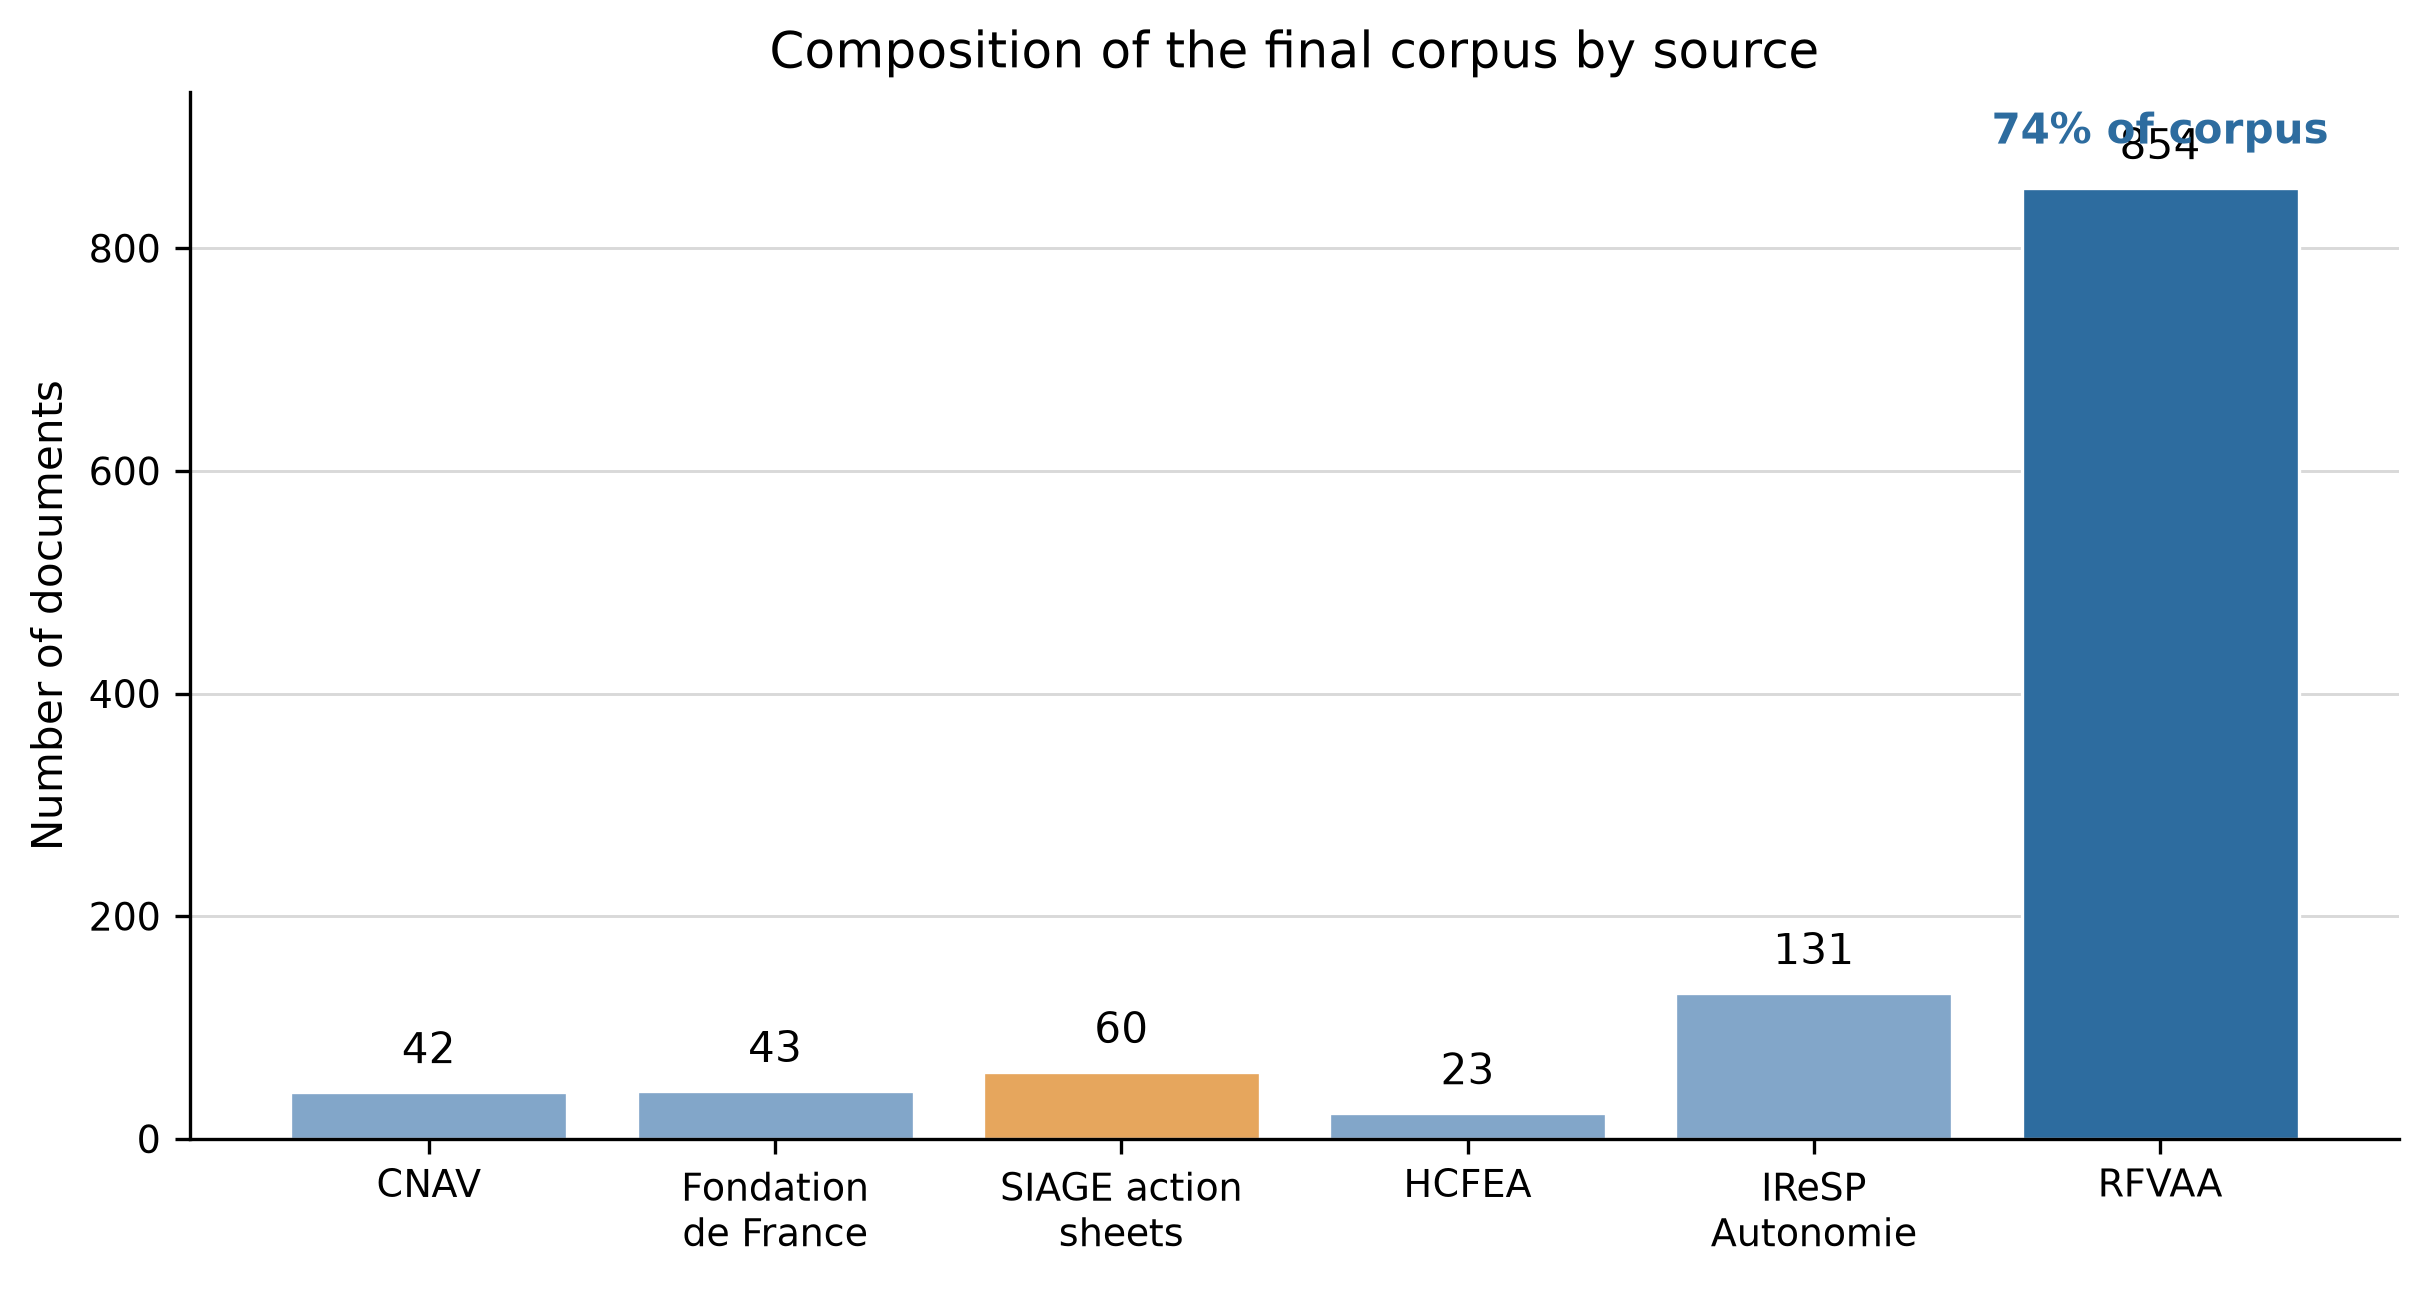
\includegraphics[width=0.98\textwidth]{Figures/corpus-source-composition.png}
    \caption{Composition of the final corpus by source. RFVAA accounts for
    854 of the 1,153 documents (approximately 74\%); descriptive results
    should therefore be interpreted in light of this source imbalance.}
    \label{fig:corpus-source-composition}
\end{figure}

Several other websites were considered during the exploration phase, including
France Bénévolat, Fondation La Poste, Fondation Nicolas Hulot, AGURAM, and
Villages d'Avenir. They were not retained for automated collection because they
contained too few exploitable documents, insufficiently structured information,
or resources that were difficult to access and process automatically.

The corpus is not a statistically representative sample of all French
initiatives related to ageing. RFVAA contributes 854 of the 1,153 records, or
approximately 74\% of the corpus. This source imbalance must be considered when
interpreting descriptive statistics: the most frequent themes, initiative types,
or stakeholders may partly reflect the editorial coverage of RFVAA rather than
the full French landscape of territorial adaptation.

\section{Cleaning and preprocessing}

After collection, the raw text files require preprocessing before they can be
analysed. The source documents contain formatting noise arising from HTML
extraction, PDF conversion, duplicated page headers, fragmented lines,
inconsistent whitespace, and variable punctuation. The cleaning stage aims to
reduce these superficial differences while preserving the linguistic content and
the traceability of the original resource.

The cleaning operations include whitespace and line-ending normalisation, the
removal of obvious formatting artefacts, and file-name standardisation. The
resulting files are stored separately from the raw documents in the
\texttt{Cleaned\_Database} directory. This separation makes it possible to
repeat the cleaning process, compare original and transformed versions, and
avoid overwriting source material.

In addition to cleaning, a keyword-based relevance score was implemented as a
first quality-control mechanism. The score is not intended to classify documents
automatically as relevant or irrelevant. Instead, it identifies documents that
should be inspected first because their content appears unusually central or
peripheral to the project scope.

The score relies on weighted keywords associated with ageing and territorial
adaptation. Higher weights are assigned to specific concepts directly related to
the project, whereas broader contextual terms receive lower weights.

\begin{table}[H]
\centering
\begin{tabular}{lc}
\toprule
Keyword & Weight \\
\midrule
agisme & 5 \\
ville amie des aines & 5 \\
vada & 5 \\
vieillissement & 3 \\
personnes agees & 3 \\
aine & 3 \\
seniors & 3 \\
retraites & 3 \\
vieillir & 3 \\
retraite & 3 \\
age & 3 \\
intergenerationnel & 3 \\
chez soi & 1 \\
ehpad & 1 \\
mobilite & 1 \\
hebergement & 1 \\
autonomie & 1 \\
citoyen & 1 \\
fragile & 1 \\
vulnerable & 1 \\
dependant & 1 \\
isole & 1 \\
aidant & 1 \\
\bottomrule
\end{tabular}
\caption{Keyword weighting used for relevance scoring.}
\label{tab:keyword-weights}
\end{table}

For each document, the script counts the occurrences of these keywords in the
normalised text and applies a small bonus if a keyword appears in the file name.
The resulting score is normalised by the number of words in the document to make
documents of different lengths more comparable. The scripts produce ranked lists
of documents with the highest and lowest scores. Low-ranked documents can be
inspected for irrelevant or poorly extracted content; high-ranked documents
provide a quick check that the corpus includes strongly relevant resources.

This relevance score is therefore a tool for quality control and manual-review
prioritisation. It must not be interpreted as a supervised classifier, a
validated measure of relevance, or an evaluation of the factual quality of the
subsequent metadata extraction.

\section{Progressive structuring of the document database}

The project architecture uses distinct directories for each major transformation.
This modular design makes it possible to isolate a processing stage, inspect its
outputs, and identify where an error was introduced. The organisation of the
project is summarised below.

\begin{verbatim}
Index_Insight/
|-- Database/
|-- Cleaned_Database/
|-- Segmented_Database/
|-- Sectioned_Database/
|-- Entities_Database/
|-- Candidates_Database/
|-- Scored_Database/
|-- Final_Tagged_Database/
|-- LLM_Tagged_Database/
|-- Evaluation/
|-- outputs_graphs/
|-- Scripts/
|-- temp/
|-- venv/
\end{verbatim}

The \texttt{Database} directory contains raw collected text files. The
\texttt{Cleaned\_Database} contains their normalised versions. The first
experimental rule-based pipeline then produces several intermediate databases.

The \texttt{Segmented\_Database} stores paragraphs, lines, and sentences. This
representation is useful because relevant information may be expressed at
different textual levels. The \texttt{Sectioned\_Database} adds detected
document sections, for example sections corresponding to objectives, target
publics, context, stakeholders, dates, or territorial information when explicit
headings are present.

The \texttt{Entities\_Database} stores intermediate entity-extraction results.
The \texttt{Candidates\_Database} contains candidate values identified for
metadata fields. The \texttt{Scored\_Database} associates these candidates with
heuristic scores and confidence values. Finally, the
\texttt{Final\_Tagged\_Database} consolidates the selected values into a
structured rule-based JSON representation and produces a global JSON file.

This progressive pipeline has two main advantages. First, it provides
transparency: intermediate candidate values and scores can be inspected rather
than treating extraction as a single opaque operation. Second, it supports
debugging and iterative development. Its limitation is that manually designed
rules do not generalise easily across the full diversity of documents.

\section{LLM-assisted structured extraction}

To address the limitations of exclusively rule-based extraction, the project
progressively adopted prompt-based structured information extraction. The
\texttt{LLM\_Tagged\_Database} directory stores JSON records generated by a
local language model. Each record corresponds to one source document and
contains structured metadata extracted from the text.

The current RFVAA extraction script uses the local model
\texttt{qwen2.5:1.5b} through the Ollama chat API. Local inference was selected
to avoid dependence on an external commercial API, maintain control over the
processing workflow, reduce operational costs, and permit iterative prompt
experimentation. If another model generated all or part of the final database,
the model identifier and the scope of that use must be reported explicitly in
the final version of the thesis.

For every document, the extraction script dynamically constructs a French prompt
that specifies the expected JSON keys, the constraints of each field, and
controlled vocabularies. The model is instructed to produce only valid JSON,
without Markdown or explanatory text, not to invent information, and to use an
empty string or an empty list when the document does not support a reliable
value.

The expected schema contains the following fields:

\begin{itemize}
    \item \texttt{titre};
    \item \texttt{territoire};
    \item \texttt{echelle};
    \item \texttt{public\_vise};
    \item \texttt{nature\_initiative};
    \item \texttt{description\_generale};
    \item \texttt{contexte};
    \item \texttt{problematique};
    \item \texttt{solution\_envisagee};
    \item \texttt{objectifs};
    \item \texttt{porteur\_initiative};
    \item \texttt{date};
    \item \texttt{thematique};
    \item \texttt{source\_site}.
\end{itemize}

These fields constitute the initial extraction schema. The original LLM values
for \texttt{thematique} and \texttt{nature\_initiative} are subsequently
preserved and complemented by normalised fields intended for filtering and
descriptive analysis.

Several fields rely on controlled vocabularies to reduce avoidable variation.
For example, \texttt{public\_vise} is constrained to values such as
\textit{aînés}, \textit{aînés et autres}, \textit{professionnels},
\textit{autre}, or \textit{public non connu}. The field \texttt{echelle} is a
list restricted to \textit{quartier}, \textit{communale},
\textit{intercommunale}, \textit{départementale}, \textit{régionale},
\textit{nationale}, and \textit{internationale}. The model is also asked to use
short and homogeneous labels for themes and initiative types.

The current configuration uses a temperature of 0, a context window of 8,192
tokens, a maximum prediction length of 700 tokens, and an input truncation
threshold of 2,500 characters in the RFVAA extraction script. The deterministic
temperature helps make successive executions more stable. However, the
truncation threshold is a limitation because information located late in a long
document may not be sent to the model.

The extraction pipeline can be summarised as follows:

\begin{center}
Raw source $\rightarrow$ text extraction $\rightarrow$ cleaning and inspection
$\rightarrow$ constrained prompt $\rightarrow$ local LLM $\rightarrow$
structured JSON $\rightarrow$ statistics and manual review.
\end{center}

Raw model responses are archived when available. This provides an audit trail:
an unexpected value can be compared with both the prompt and the model answer.
The JSON records are also checked before use, and records that cannot be parsed
or do not satisfy the expected structure can be flagged for reprocessing or
manual inspection.

The LLM approach improves flexibility when document structures vary, but it
does not eliminate the need for validation. Outputs can contain ambiguous
interpretations, unsupported inferences, inconsistent categories, or formatting
errors. The quality of an output depends on source quality, prompt design, model
version, and the part of the document made available to the model.

\section{Post-extraction taxonomy normalisation}

Although the extraction prompt encourages short and homogeneous labels, the
fields \texttt{thematique} and \texttt{nature\_initiative} may still contain
lexical variants that refer to closely related concepts. For example, labels
such as \textit{lien social}, \textit{isolement}, and \textit{inclusion sociale}
cannot be compared reliably if they are treated as unrelated categories. A
deterministic post-processing step was therefore implemented to complement the
LLM output with controlled, documented categories.

The original fields \texttt{thematique} and \texttt{nature\_initiative} remain
unchanged. The normalisation script adds the fields
\texttt{thematique\_normalisee},
\texttt{nature\_initiative\_normalisee}, and
\texttt{version\_taxonomie}. This separation preserves the original wording
generated from the source document while providing consistent labels for
filtering, statistics, and visualisation.

The thematic taxonomy contains fifteen substantive categories:
\textit{autonomie et avancée en âge}, \textit{santé et prévention},
\textit{aidants, handicap et vulnérabilités}, \textit{lien social et lutte
contre l'isolement}, \textit{intergénérationnel}, \textit{mobilité et
accessibilité}, \textit{habitat et logement}, \textit{numérique et accès à
l'information}, \textit{participation citoyenne et gouvernance},
\textit{culture et loisirs}, \textit{activité physique et sport},
\textit{espaces publics et aménagement}, \textit{services et
accompagnement}, \textit{politiques publiques et recherche}, and
\textit{environnement et développement durable}. A record may receive several
normalised themes when its original labels explicitly refer to several
dimensions.

The initiative-type taxonomy includes \textit{atelier}, \textit{formation},
\textit{sensibilisation}, \textit{enquête ou étude}, \textit{rapport ou
publication}, \textit{plaidoyer}, \textit{outil numérique},
\textit{événement}, \textit{accompagnement}, \textit{dispositif ou
programme}, \textit{offre de service}, \textit{groupe de parole},
\textit{consultation citoyenne}, \textit{lieu ou espace dédié}, and
\textit{projet d'aménagement}. Unlike themes, each record receives one
normalised initiative type.

The normalisation is rule-based and does not call the LLM again. It operates on
the extracted labels rather than on the full source text, making the
transformation reproducible and inspectable. Values that cannot be mapped
unambiguously are assigned to \textit{autre / à revoir} and listed in a review
report. This conservative design avoids masking uncertainty behind an overly
broad automatic category and allows the taxonomy to be refined through
documented manual review.


\section{Indexing, exploration, and analytical outputs}

One objective of the project is to make the corpus easier to explore and compare.
Without structured metadata, the corpus would remain a collection of independent
text files that are difficult to navigate manually. The normalised metadata make
it possible to access consistent thematic and initiative-type categories
directly, rather than parsing the full text for every query or treating minor
lexical variations as distinct concepts.

The structured corpus can support several forms of documentary exploration:

\begin{itemize}
    \item keyword-based search in titles and descriptions;
    \item metadata filtering by source, territorial scale, target audience, or
    initiative type;
    \item thematic exploration;
    \item territorial comparison;
    \item comparison between SIAGE action sheets and other documents;
    \item navigation through stakeholders, dates, and initiative categories.
\end{itemize}

The project also contains scripts that create spreadsheets and charts from the
LLM-tagged records. These outputs include distributions of themes, initiative
types, stakeholders, territories, temporal mentions, and comparisons between
action sheets and other documents. Cost-related information is also extracted
exploratorily when it can be identified in the records.

At the current stage, the indexing system remains a structured prototype rather
than a fully operational search engine. The project produces machine-readable
JSON data and analytical outputs, but does not yet deploy a dedicated retrieval
engine, vector database, or public web interface. Consequently, the thesis
should describe semantic retrieval, embeddings, FAISS, Elasticsearch, and
interactive interfaces as future possibilities rather than as implemented
features.

Future work could include semantic search based on embeddings, hybrid retrieval
combining lexical and semantic methods, clustering of initiatives according to
thematic proximity, recommendation of similar initiatives, and an interactive
interface designed with the future users of the INSIGHT project.

\section{Analytical questions and interpretation framework}

Beyond the technical objective of structuring the corpus, the project supports
an exploratory analysis of territorial responses to population ageing. The
following questions guide this analysis:

\begin{enumerate}
    \item What are the principal types of initiatives described in the corpus?
    \item How do these types vary according to thematic domain, territorial
    scale, target audience, and initiative holder?
    \item What roles are attributed to workshops in the documents, compared with
    other forms of response such as services, digital tools, training,
    awareness-raising activities, or territorial planning projects?
    \item To what extent are dates and cost information available, structured,
    and comparable across sources?
\end{enumerate}

These questions are exploratory. The corpus documents initiatives that were
collected from selected sources; it does not provide a representative survey of
all initiatives in France, nor does it measure their effectiveness. The analysis
therefore describes how initiatives are represented in the corpus and does not
establish causal claims about their impact.

\subsection{Typology of territorial responses}

The field \texttt{nature\_initiative} makes it possible to distinguish several
forms of response to ageing-related challenges, including workshops, training,
awareness-raising activities, services, support schemes, digital tools, events,
publications, discussion groups, dedicated places, and planning projects. This
typology can be analysed jointly with \texttt{thematique},
\texttt{public\_vise}, \texttt{echelle}, and \texttt{porteur\_initiative}.
For example, it can indicate whether certain response types are more often
associated with social connection, health prevention, housing, mobility, or
digital inclusion, and whether they are mainly carried by public institutions,
associations, or local authorities.

The objective is not to rank these response types. It is to make visible the
diversity of intervention formats and to identify the combinations of problems,
publics, actors, and territorial scales that occur in the collected material.

\subsection{Interpreting the prominence of workshops}

If workshops are frequent in the corpus, this can be investigated by comparing
their thematic distribution, target publics, objectives, and stated
problematiques with those of other initiative types. The analysis can identify
the functions attributed to workshops in the documents: for instance,
prevention, information, acquisition of practical knowledge, social connection,
peer exchange, participation, or the identification of local needs.

However, frequency does not demonstrate effectiveness. The corpus generally
describes the intended function or expected benefit of a workshop; it does not
systematically contain outcome measures or control groups. The thesis should
therefore formulate conclusions as follows: workshops are represented as a
particular type of response and are associated with particular intended
mechanisms, rather than claiming that they produce a proven effect.

\subsection{Temporal and cost information}

The date field contains temporal expressions mentioned in the documents. A
frequent year, such as 2019, may refer to the start of an initiative, a
publication date, a funding period, an event date, or a date cited in the
description. It should not automatically be interpreted as the year when an
initiative began. A temporal analysis is meaningful only after distinguishing,
where possible, the semantic role of each date and reporting the proportion of
records for which this role remains uncertain.

Cost information can provide an additional exploratory perspective. The project
contains a dedicated extraction procedure for cost-related mentions, but these
values may refer to a total budget, a grant, a cost per participant, a duration,
or an amount not directly associated with the initiative. Before comparing
amounts, the analysis should report the coverage rate, currency, unit, year,
and semantic type of each value. Costs should therefore be presented as
documented information available for a subset of the corpus, not as a complete
or directly comparable economic evaluation.

\subsection{NLP and interdisciplinary contribution}

The contribution of natural language processing to this project is not to
replace social-science interpretation. Its role is to make a large, fragmented,
and heterogeneous documentary corpus tractable: it supports systematic
collection, structured description, filtering, comparison, and the
identification of patterns that would be difficult to observe by reading more
than one thousand documents individually.

The interdisciplinary value of the project arises from this complementarity.
Research on ageing, territorial policies, participation, and social inclusion
provides the concepts needed to interpret the data. NLP provides the technical
means to organise and explore the material at scale. Interpretation, category
validation, and the assessment of policy relevance remain human and
context-dependent tasks.

\section{Methodological limits}

Several limits must be considered when interpreting the corpus and the outputs.
First, the corpus is unevenly distributed across sources, with RFVAA strongly
represented. Second, raw web and PDF extraction may preserve boilerplate text, incomplete
metadata, duplicate passages, or encoding artefacts. Third,
territorial references can refer to a location, an organisation, or a project
area, while the initiative holder can be confused with a partner or funder.

Controlled vocabularies reduce output variability but may hide
meaningful distinctions between initiatives. Finally, a populated metadata field
is not necessarily factually correct. Automatic completion and rule-based
confidence indicators are useful for quality control, but they do not replace a
human reference evaluation. The next chapter therefore distinguishes technical
coverage from factual extraction accuracy and presents the evaluation strategy.

\chapter{Implementation}

\section{Development environment and reproducibility}

The pipeline was developed in Python in an isolated virtual environment. Its
dependencies cover HTTP collection, HTML parsing, PDF extraction, JSON and CSV
processing, spreadsheet production, and plotting. LLM inference is provided
locally by Ollama. The project is organised as a collection of independent
scripts rather than as a single monolithic application, so that collection,
cleaning, extraction, evaluation, and analysis can be executed and inspected
separately.

Reproducibility requires recording the Python version, package versions, Ollama
version, model identifier, execution date, prompt version, and inference
parameters. The core workflow does not rely on an external commercial LLM API.
However, reproducibility is not perfect across machines: a model update, changed
source page, or modified prompt can alter outputs. Raw input text, generated
JSON, archived raw LLM answers, and collection indexes are therefore retained as
provenance artefacts.

The project directory separates raw data, cleaned data, intermediate
representations, structured outputs, evaluation material, and analysis outputs.
This organisation prevents a processing step from silently overwriting its
input. It also makes it possible to rerun one stage after a correction without
having to repeat the whole workflow. For example, changes to the taxonomy
normalisation can be applied to existing JSON records without downloading the
corpus again or running new LLM inferences.

\section{Project architecture and data flow}

The implementation follows a file-based architecture. Each source document is
represented by one text file and, after extraction, by one JSON record with the
same logical identity. Dedicated directories store the successive
representations: \texttt{Database} for collected text, \texttt{Cleaned\_Database}
for normalised text, several intermediate directories for the experimental
rule-based pipeline, and \texttt{LLM\_Tagged\_Database} for LLM-generated
records. This one-document-per-file principle simplifies error localisation:
when a value appears incorrect, the corresponding JSON output can be compared
directly with the cleaned text and, where available, the raw model response.

Collection scripts are source-specific because the corpus includes HTML pages,
PDF files, internal action sheets, and research-project records with different
structures. They retrieve the source content, extract or convert it to text,
and maintain an index containing information such as the title, local filename,
and source URL when available. The cleaning scripts then reduce formatting noise
caused by HTML extraction and PDF conversion, including duplicated headers,
fragmented lines, inconsistent whitespace, and filename variations.

The initial rule-based pipeline was implemented as a sequence of modules for
segmentation, section detection, entity extraction, candidate extraction,
heuristic scoring, JSON consolidation, and review-table generation. Each module
writes an intermediate output rather than passing data only in memory to the
next stage. This design was useful for debugging and for understanding the
effect of individual rules, even though the final extraction workflow relies
primarily on constrained LLM extraction.

\section{LLM extraction and output validation}

The LLM module constructs a French prompt for each document and submits it to
the local Ollama chat API. The prompt specifies the required JSON keys, the
expected data types, controlled vocabularies for selected fields, and the
instruction not to invent unsupported information. The model is asked to return
an empty string or an empty list when the document does not provide a reliable
value. The configuration uses the local \texttt{qwen2.5:1.5b} model, a
temperature of 0, a context window of 8,192 tokens, a maximum generation length
of 700 tokens, and an input limit of 2,500 characters for the RFVAA extraction
script.

Structured generation does not guarantee that every response is immediately
usable. The implementation therefore includes defensive processing before a
record is saved. It removes text outside the JSON object when present, repairs
superficial formatting issues such as typographic quotation marks or trailing
commas, and attempts to parse the result. Records that remain invalid can be
flagged for reprocessing or manual inspection rather than being silently merged
into the final dataset. Where available, the unmodified model response is saved
alongside the structured record, which permits later inspection of a parsing
problem or an unexpected extraction.

The resulting JSON records preserve both extracted metadata and contextual
descriptions. They include title, territory, territorial scale, target
audience, initiative type, initiative holder, dates, themes, and source
identification, together with short descriptive fields. The schema is designed
for documentary exploration rather than to claim that every field is known for
every source. Empty values are therefore meaningful: they represent missing or
insufficiently supported information, not a processing failure by default.

\section{Provenance and taxonomy normalisation}

Two deterministic post-processing components complement the LLM extraction.
First, the provenance script adds \texttt{source\_site}, \texttt{source\_url},
\texttt{original\_title}, and \texttt{collection\_date} to every available JSON
record using collection indexes and archived source files. These values are not
generated by the LLM. The script reports coverage by source and leaves a field
empty when a reliable value is unavailable. In particular, the SIAGE action
sheets are marked as internal material and do not receive an artificial public
URL. Historical collection dates are also left empty because they were not
consistently recorded in the original indexes.

Second, a taxonomy-normalisation script adds
\texttt{thematique\_normalisee} and
\texttt{nature\_initiative\_normalisee}, while preserving the original LLM
fields. The implementation maps lexical variants to a documented French
controlled taxonomy so that related labels can be aggregated consistently in
filters and charts. It does not invoke the LLM again. Ambiguous values are
assigned to \textit{autre / à revoir} and written to a review report instead of
being forced into an unsuitable category. The records also store a taxonomy
version, allowing later revisions to be identified and reapplied.

\section{Main modules and outputs}

The main modules can be grouped into five functional families:

\begin{itemize}
    \item source-specific collection scripts for CNAV, Fondation de France,
    HCFEA, IReSP, RFVAA, and the SIAGE action sheets;
    \item cleaning, file-name standardisation, segmentation, and
    keyword-based relevance-scoring scripts;
    \item rule-based extraction modules that generate intermediate candidates,
    scores, consolidated records, and review tables;
    \item local LLM extraction, JSON repair, taxonomy normalisation, and
    provenance-enrichment scripts;
    \item evaluation and analysis scripts that create reference samples,
    calculate scores, and produce spreadsheets and charts.
\end{itemize}

The principal output is a collection of JSON records usable by downstream
software. Complementary outputs include a consolidated JSON file, CSV review
tables, Excel workbooks, and charts describing themes, initiative types,
stakeholders, territories, temporal mentions, and comparisons between SIAGE
action sheets and other documents. The current analytical scripts prioritise
the normalised theme and initiative-type fields when available, while retaining
the original values for audit and correction. These outputs are exploratory;
they do not estimate the real-world frequency or effectiveness of initiatives
in France.

\section{Difficulties and implemented solutions}

Structural heterogeneity was the main implementation difficulty: a heading in
one source can be expressed as a paragraph, table, caption, or be absent in
another. The modular pipeline and the separation between raw, cleaned, and
intermediate directories made this variability inspectable. The transition from
rule-based extraction to constrained LLM extraction reduced the need for a
large number of source-specific rules, while controlled vocabularies and
post-extraction normalisation limited avoidable output variation.

Several difficulties remain. PDF conversion can introduce encoding artefacts or
reading-order errors, and websites may change their structure after collection.
Dates can refer to publication, funding, event, or initiative-start dates;
territorial references can refer to a place, an organisation, or a project
area; and an organisation mentioned in a document is not necessarily the
initiative holder. The system therefore retains source links, original titles,
raw texts, and intermediate outputs so that these cases can be reviewed. The
human reference evaluation described in the next chapter provides a separate
assessment of factual extraction quality; the implementation itself does not
treat field completion as evidence of correctness.

\chapter{Evaluation}

\section{Evaluation objectives}

The evaluation has two distinct objectives. The first concerns technical
usability: records should be valid, fields should be populated, and provenance
should be retained. The second concerns factual extraction quality: a populated
field must be correct and supported by the source text. These objectives must
not be confused, since a complete record can still contain an incorrect or an
overly inferred value.

\section{Automatic coverage results}

The rule-based consolidated database contains 1,153 records. Its review table
measures field completion and an internal heuristic confidence score. The
results in Table~\ref{tab:coverage-results} demonstrate high field population,
but neither measure is a human-judged accuracy score nor a measure of LLM
performance.

\begin{table}[H]
\centering
\begin{tabular}{lrrr}
\toprule
Source & Records & Mean completion rate & Mean heuristic confidence \\
\midrule
CNAV & 42 & 0.99 & 0.58 \\
Fiches actions SIAGE & 60 & 0.94 & 0.53 \\
Fondation de France & 43 & 0.97 & 0.58 \\
HCFEA & 23 & 0.97 & 0.54 \\
IReSP Autonomie & 131 & 0.98 & 0.63 \\
RFVAA & 854 & 1.00 & 0.60 \\
\midrule
Overall & 1,153 & 0.99 & 0.59 \\
\bottomrule
\end{tabular}
\caption{Automatic coverage of the rule-based consolidated database.}
\label{tab:coverage-results}
\end{table}

Completion covers title, territory, scale, target audience, stakeholder, date,
theme, source, and five descriptive fields. The confidence figure derives from
rule-based candidate scores. It is useful for prioritising manual review, not as
a calibrated probability that a field is correct.

\section{Human reference evaluation protocol}

The factual quality of LLM-assisted extraction was evaluated through a manually
annotated reference sample. Sixty documents were selected using a reproducible
random draw, stratified by source: ten documents were drawn from each of the
six corpus sources. This equal allocation was chosen to ensure that small
sources were represented in the evaluation; it does not reproduce the source
distribution of the complete corpus.

For each selected document, the LLM output was compared with its cleaned source
text. Seven fields were examined: \texttt{territoire}, \texttt{echelle},
\texttt{public\_vise}, \texttt{nature\_initiative},
\texttt{porteur\_initiative}, \texttt{date}, and \texttt{thematique}.
For the categorical fields \texttt{public\_vise},
\texttt{echelle}, and \texttt{nature\_initiative}, the annotator recorded a
reference value and the evaluation reports micro precision, recall, micro F1,
macro F1, and exact-match rate. For the remaining fields, each model output was
judged as \textit{correct}, \textit{partiel}, \textit{incorrect},
\textit{absence correcte}, or \textit{non \'{e}valuable}. A prediction was
considered correct only when it was explicitly supported by the source text.

The labels \textit{absence correcte} and \textit{non \'{e}valuable} describe
two different situations. \textit{Absence correcte} was assigned when the model
left a field empty and the source text did not provide enough information to fill
it reliably; this is treated as a successful prediction. In contrast,
\textit{non \'{e}valuable} was assigned when the reviewer could not establish a
reliable reference value because the source text was too ambiguous, incomplete, or
degraded. Non-evaluable cases are reported separately and excluded from the
denominator of the accepted rate.

The annotation was performed by one reviewer. Consequently, the results
measure agreement with this documented reference annotation, but do not provide
an inter-annotator agreement estimate. A second independent annotation of a
subset would be a useful extension.

\section{Human reference evaluation results}

Table~\ref{tab:llm-categorical-results} reports the results for the three
categorical fields evaluated against reference labels. All scores range from 0 to 1, with 1 indicating
perfect agreement with the reference annotation. Precision measures whether the
labels produced by the model were appropriate; recall measures whether the labels
expected from the source text were retrieved; and exact match requires the full
predicted value to match the reference value for a document.

The target-audience field was evaluated against the French controlled vocabulary
used in the extraction prompt: \textit{aînés}, \textit{aînés et autres},
\textit{professionnels}, \textit{autre}, and \textit{public non connu}. The model
achieved perfect scores in this sample for target audience and initiative type.
Territorial scale produced one non-exact prediction. In this case, the reference
label was \textit{nationale}, whereas the model returned an empty value. The model
therefore introduced no incorrect scale label, which explains the
precision of 1.000, but it missed one expected label, producing a recall of 0.987.

\begin{table}[H]
\centering
\begin{tabular}{lrrrrr}
\toprule
Field & Precision & Recall & F1 micro & F1 macro & Exact match \\
\midrule
Target audience & 1.000 & 1.000 & 1.000 & 1.000 & 1.000 \\
Initiative type & 1.000 & 1.000 & 1.000 & 1.000 & 1.000 \\
Territorial scale & 1.000 & 0.987 & 0.993 & 0.993 & 0.983 \\
\bottomrule
\end{tabular}
\caption{Human reference evaluation of categorical metadata
(n=60 documents per field).}
\label{tab:llm-categorical-results}
\end{table}

Table~\ref{tab:llm-judgment-results} presents the human judgments for the
remaining fields. ``Evaluable'' is the number of documents for which the reviewer
could establish a reference value; it is therefore equal to 60 minus the number of
non-evaluable cases. ``Accepted'' combines \textit{correct} and \textit{absence
correcte} judgments. The accepted rate is calculated only on evaluable documents,
so it measures the model's factual reliability where the source permits a clear
assessment. ``Partial'' identifies a value that is broadly supported but incomplete
or overly vague, whereas ``incorrect'' identifies an unsupported or wrong value.

\begin{table}[H]
\centering
\begin{tabular}{lrrrrrr}
\toprule
Field & Evaluable & Accepted & Partial & Incorrect & Non-evaluable & Accepted rate \\
\midrule
Territory & 54 & 53 & 1 & 0 & 6 & 0.981 \\
Stakeholder & 38 & 37 & 0 & 1 & 22 & 0.974 \\
Date & 56 & 44 & 7 & 5 & 4 & 0.786 \\
Theme & 60 & 60 & 0 & 0 & 0 & 1.000 \\
\bottomrule
\end{tabular}
\caption{Human judgments of LLM metadata extraction. ``Accepted'' includes
correct predictions and correctly empty fields.}
\label{tab:llm-judgment-results}
\end{table}

\begin{figure}[H]
    \centering
    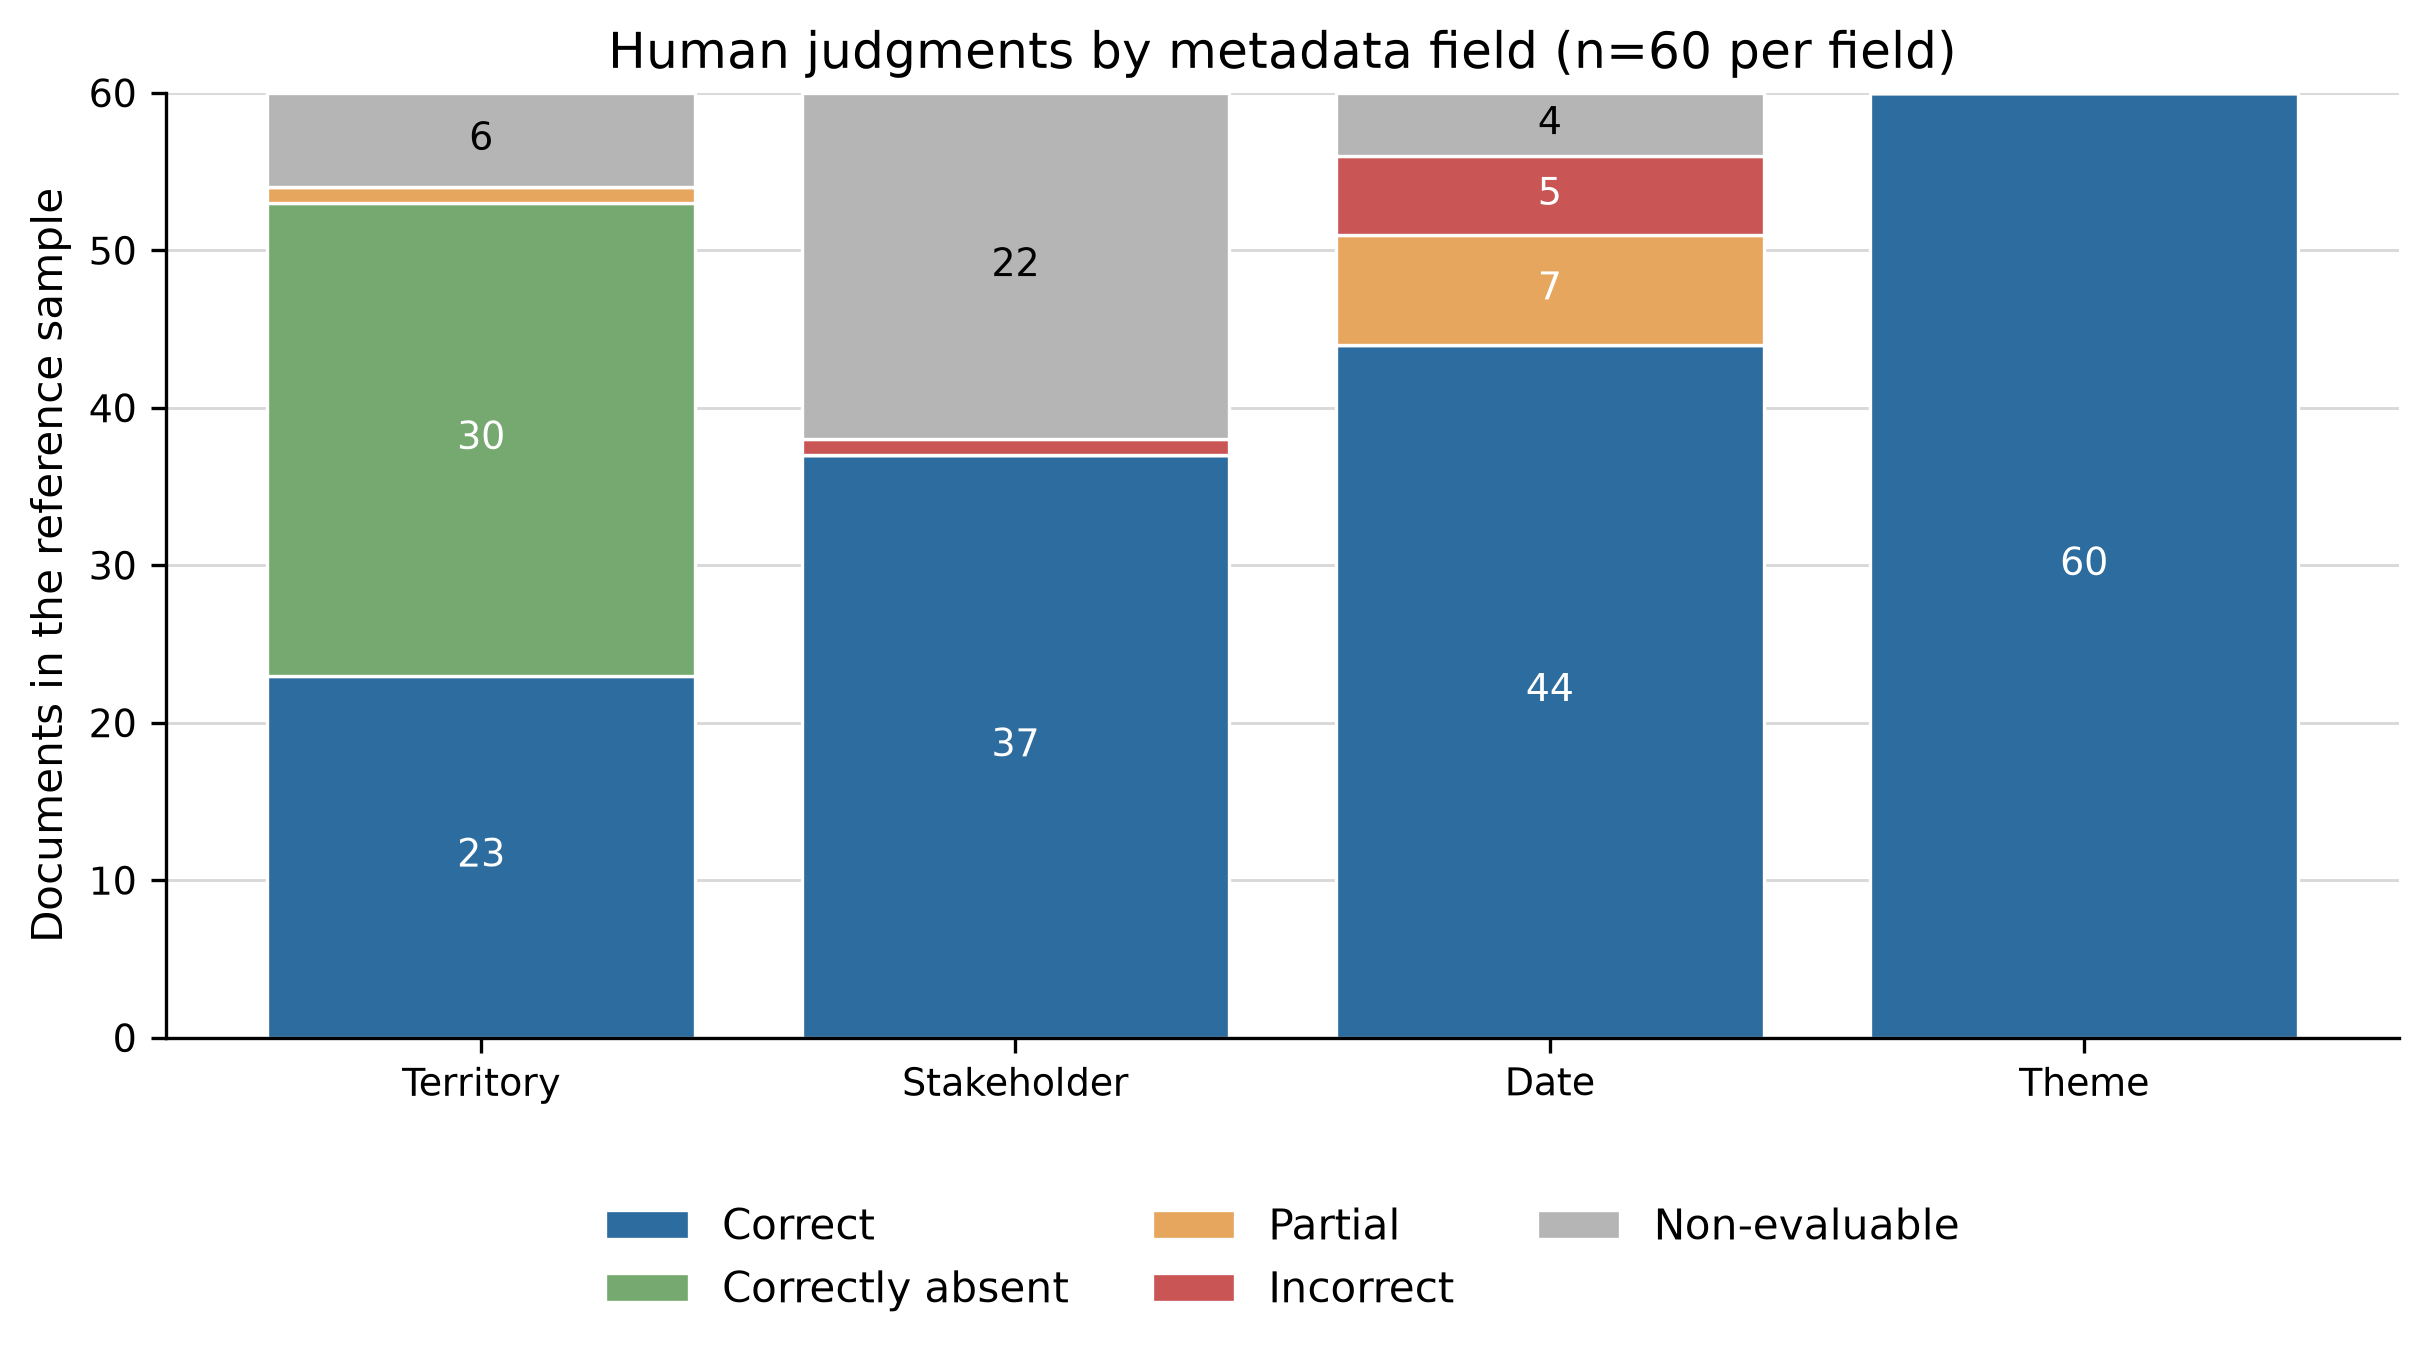
\includegraphics[width=1\textwidth]{Figures/human-judgment-distribution.png}
    \caption{Distribution of human judgments for four extracted metadata
    fields. Correctly absent predictions are treated as accepted because the
    source did not provide sufficient information to fill the corresponding
    field.}
    \label{fig:human-judgment-distribution}
\end{figure}

\subsection{Exploratory source-level analysis}

Because the reference sample contains ten documents from each source, the same
annotations can be inspected by source to identify possible sensitivity to
documentary format. This analysis is exploratory: ten documents per source are
not sufficient to estimate a stable source-specific performance level, and the
results should therefore be read as diagnostic evidence rather than as a ranking
of sources.

Target audience, initiative type, and theme were fully accepted in all six
source subsets. Territorial scale was also fully correct for five sources. The
only exception was Fondation de France, for which one expected scale label was
missed, resulting in an F1 score of 0.957. Table~\ref{tab:llm-source-results}
focuses on the fields for which source-dependent variation is most informative.
For territory, holder, and date, the notation $a/b$ gives the number of accepted
predictions over evaluable documents; ``--'' indicates that no document was
evaluable for that field.

\begin{table}[H]
\centering
\small
\begin{tabular}{lrrrr}
\toprule
Source & Scale F1 & Territory & Holder & Date \\
\midrule
CNAV & 1.000 & 8/9 (0.889) & 10/10 (1.000) & 4/8 (0.500) \\
Fiches actions SIAGE & 1.000 & 10/10 (1.000) & 8/9 (0.889) & 8/10 (0.800) \\
Fondation de France & 0.957 & 8/8 (1.000) & 7/7 (1.000) & 8/8 (1.000) \\
HCFEA & 1.000 & 9/9 (1.000) & 2/2 (1.000) & 9/10 (0.900) \\
IReSP Autonomie & 1.000 & 8/8 (1.000) & -- & 9/10 (0.900) \\
RFVAA & 1.000 & 10/10 (1.000) & 10/10 (1.000) & 6/10 (0.600) \\
\bottomrule
\end{tabular}
\caption{Exploratory source-level results from the stratified reference sample.
Territory, holder, and date are reported as accepted predictions over evaluable
documents, followed by the accepted rate.}
\label{tab:llm-source-results}
\end{table}

\subsection{Comparison with the rule-based baseline}

To assess the practical contribution of LLM-assisted extraction, the same
human-annotated reference sample was also evaluated with a deterministic
rule-based baseline. The comparison uses the same 60 documents and the same
gold labels as the LLM evaluation for \texttt{public\_vise},
\texttt{echelle}, and \texttt{nature\_initiative}. It is therefore a paired
comparison: differences cannot be attributed to a different sample or to a
different reference annotation.

For \texttt{public\_vise} and \texttt{echelle}, the baseline reuses the
outputs of the historical rule-based pipeline stored in
\texttt{Final\_Tagged\_Database}. The historical schema did not include a
\texttt{nature\_initiative} field. For this field, a documented deterministic
extension was applied to the first 2,500 characters of each cleaned document:
it assigns the first category whose predefined keyword rule matches the text.
This extension does not call an LLM. Its use makes the comparison possible,
but it should not be confused with a native output of the original rule-based
database.

\begin{table}[H]
\centering
\small
\begin{tabular}{lrrrrrr}
\toprule
& \multicolumn{3}{c}{Rule-based baseline} & \multicolumn{3}{c}{Local LLM} \\
\cmidrule(lr){2-4} \cmidrule(lr){5-7}
Field & Precision & Recall & F1 & Precision & Recall & F1 \\
\midrule
Target audience & 0.283 & 0.283 & 0.283 & 1.000 & 1.000 & 1.000 \\
Territorial scale & 0.347 & 0.436 & 0.386 & 1.000 & 0.987 & 0.993 \\
Initiative type & 0.589 & 0.550 & 0.569 & 1.000 & 1.000 & 1.000 \\
\bottomrule
\end{tabular}
\caption{Paired comparison between the deterministic rule-based baseline and
the local LLM on the 60-document human reference sample. Scores are micro
precision, recall, and F1.}
\label{tab:rule-based-llm-comparison}
\end{table}

The LLM achieved higher F1 scores for all three fields. The largest difference
appeared for target audience ($+0.717$ F1) and territorial scale ($+0.607$ F1).
The historical rule-based outputs for these fields were often free-text
candidate excerpts or over-inclusive keyword matches, whereas the LLM prompt
required a normalised target-audience label and a restricted list of territorial
scales. For initiative type, the keyword baseline reached an F1 of 0.569. It
correctly identified explicit terms such as \textit{atelier}, \textit{formation},
or \textit{rapport}, but it selected the first matching term and therefore
struggled when a document mentioned several possible forms of activity.

This result does not make the rule-based approach obsolete. Its decisions are
deterministic, easy to inspect, and useful for identifying explicit lexical
signals. However, on this heterogeneous corpus, the constrained LLM is better
able to select a field value that corresponds to the intended metadata schema.
The comparison is diagnostic rather than a definitive benchmark: it uses one
60-document, source-stratified sample and one human annotator. A larger blind
reference annotation and a second annotator would be needed to quantify the
generalisation of the observed differences.

The results suggest that date extraction is particularly dependent on source
format. The accepted date rate ranges from 0.500 for CNAV to 1.000 for
Fondation de France, with RFVAA also showing a lower rate of 0.600. This is
consistent with the different roles of temporal expressions in the sources:
they may describe an initiative, an event, a publication, or an update to a
document. The IReSP holder field was non-evaluable in all ten sampled records,
which reflects the frequent absence of a clearly identifiable initiative holder
in research-project descriptions rather than a measured model failure.

\section{Results analysis and limitations}

The human evaluation confirms that, for this stratified sample, the LLM can
produce reliable structured metadata for target audience, initiative type,
territorial scale, theme, and territory. The results should nevertheless be
interpreted as sample-level evidence rather than as a guarantee of identical
performance on every document in the corpus. In particular, the equal source
allocation makes the evaluation appropriate for detecting source-specific
weaknesses, but it is not an estimate weighted by the distribution of the
complete corpus.

Date extraction is the clearest weakness. Among the 56 evaluable documents,
only 44 predictions were fully accepted; seven were partial and five were
incorrect. This result is consistent with the heterogeneous role of dates in
the sources: a year can refer to an initiative start, publication, event,
funding period, or another temporal mention. Future versions of the schema
should distinguish the temporal expression from its semantic role, for example
by separating publication date, initiative start date, and event date.

The stakeholder field has a high accepted rate among evaluable documents
(0.974), but 22 of the 60 documents were non-evaluable. This does not
necessarily indicate a model error; rather, many source texts do not clearly
distinguish the initiative holder from a partner, funder, or organisation merely
mentioned in the document. The interface should therefore preserve uncertainty
and provenance instead of presenting every extracted stakeholder as an
established fact.

These findings complement, rather than replace, automatic coverage measures.
The completed reference evaluation establishes factual evidence for the seven
reviewed metadata fields, while the remaining free-text descriptions still
require separate qualitative validation before being used as factual claims.
The modest sample size and the absence of a second annotator remain limitations.
Future work should extend the reference set, measure inter-annotator agreement,
and evaluate whether prompt or model changes improve the date and stakeholder
fields.

\chapter{Discussion}

\section{Contributions of the internship}

This internship delivers a documented corpus of 1,153 French-language
resources on territorial adaptation to ageing, containing approximately
917,554 word tokens. It brings together heterogeneous material from six
institutional and associative sources: CNAV, Fondation de France, SIAGE,
HCFEA, IReSP Autonomie, and the French Network of Age-friendly Cities
(RFVAA). Beyond the corpus itself, the project provides a traceable data
architecture that preserves raw documents, intermediate files, structured
records, and review artefacts.

The work also proposes a practical natural language processing workflow for a
documentary context in which sources differ substantially in form and level of
detail. A transparent rule-based baseline is complemented by a local LLM-based
extractor with a constrained French prompt and JSON output. The resulting
records can be explored through fields such as target audience, initiative
type, theme, territorial scale, territory, holder, and date. A deterministic
normalisation layer then maps the extracted themes and initiative types to
controlled French vocabularies while retaining the original model outputs.

Finally, the internship makes the resulting index more auditable. Each
structured record is associated, where available, with provenance fields such
as the source site, source URL, original title, and collection date. This
distinction between extracted metadata and documentary provenance is important:
the former supports exploration, whereas the latter allows a user to return to
the source and verify an interpretation. The project should therefore be seen
as both an NLP prototype and a documented foundation for a future INSIGHT
index.

\section{Interpretation of the extraction results}

The human review of a stratified sample of 60 documents provides evidence that
the constrained extraction workflow is usable for several fields, but it does
not establish perfect reliability for the whole corpus. In particular, the
three categorical fields evaluated against reference labels obtained very high
agreement: target audience and initiative type reached a micro-F1 of 1.000,
while territorial scale reached a micro-F1 of 0.993. Theme labels were assessed
separately through human judgment and were accepted for all 60 reviewed
documents. These results are consistent with the fact that restricted label
sets reduce output variation and make both automatic parsing and manual
assessment easier.

The open-text fields require a more nuanced reading. On evaluable cases,
accepted rates were 0.981 for territory, 0.974 for initiative holder, and
0.786 for date. These figures should not be interpreted as an intrinsic
property of the model alone. They reflect the interaction between the model,
the prompt, the extraction limit, and--above all--the evidence available in the
source documents. A holder or date may be absent, implicit, or ambiguous in a
document. For this reason, the annotation protocol distinguished an incorrect
answer from a correct absence: when the source did not provide a reliable value
and the system returned an empty field, this was considered an accepted
outcome. Conversely, non-evaluable cases were excluded from the denominator
because the source did not allow a confident human decision either.

The source-level analysis further shows why an aggregate score is not
sufficient. The controlled fields were stable across the six subsets, whereas
the date field varied more strongly according to source format. For example,
dates were less often accepted in the CNAV and RFVAA subsets than in sources
whose documents expose publication dates more consistently. Territorial scale
also missed one label in the Fondation de France subset. These results do not
demonstrate that one source is inherently more difficult than another: each
subset contains only ten documents. They nevertheless identify concrete
priorities for improvement, particularly a clearer temporal schema and
source-specific checks for fields that are often incomplete.

Overall, the experiment supports the use of the metadata as an exploratory and
reviewable index. It does not justify presenting every extracted value as a
verified fact, nor does it replace human judgement for public-facing
publication or policy analysis. The evaluation is best understood as a first
benchmark that can be extended with further annotations, a second annotator,
and agreement measures between annotators.

\section{Interpretation of descriptive outputs}

The normalised records make it possible to describe the documentary collection
and to compare subsets of documents. The most frequent thematic labels include
\textit{autonomie et avanc\'ee en \^age}, \textit{sant\'e et pr\'evention}, and
\textit{lien social et lutte contre l'isolement}. Among initiative types,
workshops, training, studies or surveys, awareness-raising activities, and
events are recurrent. These patterns are plausible in a corpus devoted to
adaptation to ageing, but they must be read as properties of the collected and
labelled documents rather than as estimates of the real distribution of
initiatives in France.

Several mechanisms can influence these descriptive outputs. First, the corpus
is highly unbalanced across sources: RFVAA documents represent the largest
share of the collection. Second, the same initiative may be documented by more
than one resource, whereas other initiatives may have little or no web
presence. Third, source editors decide which activities to publish and how to
describe them. Finally, a single document can receive several themes or
initiative types; category counts are therefore not mutually exclusive.

The normalisation step improves comparability without eliminating these
limitations. It applies deterministic mappings to the original extracted
labels, so it does not create a second model prediction. However, any
controlled vocabulary necessarily groups together some distinctions present in
the source material. The preservation of the original fields, the use of an
\textit{autre / \`a revoir} category, and versioning of the taxonomy are thus
important safeguards. In this context, the figures and tables generated by the
project are most useful for exploratory navigation, hypothesis generation, and
discussion with INSIGHT users. They should not be used to rank territories,
assess local performance, or infer causal effects.

\section{Ethical, legal, and methodological considerations}

The corpus is composed of publicly accessible institutional and associative
resources, supplemented by SIAGE action sheets supplied within the internship
context. Its purpose is documentary analysis; the system does not profile
individuals and must not be used to make consequential decisions about people,
organisations, or territories. Public accessibility is not equivalent to an
unlimited right of reuse. Collection and dissemination must remain compatible
with the terms of access of the source websites, intellectual-property rights,
database rights where applicable, and data-protection obligations
\cite{cnil2024reuse}.

Provenance is consequently both a technical and an ethical requirement. When a
document comes from an external website, the index should retain its source
site and URL, as well as its original title. This makes attribution possible,
allows corrections to be traced back to their origin, and enables a user to
consult the source rather than treating the extracted metadata as a substitute
for it. In a future public interface, the index should preferentially expose
short metadata and links to the original resource, rather than redistributing
full documents without a clear legal basis.

The use of an LLM also requires calibrated claims. Structured outputs can be
wrong, incomplete, or overly confident even when they are syntactically valid.
The project mitigates this risk through controlled vocabularies, raw-output
archiving, provenance fields, and manual evaluation. These measures improve
auditability, but human review remains necessary before metadata are published
as factual statements. This is particularly important for territories, holders,
and dates, for which the source evidence can be ambiguous.

The project also has an environmental dimension. Local inference avoids
transmitting document content to a commercial remote API, but it does not make
the workflow impact-free. Energy use depends on the hardware, model, number of
requests, and repeated experimentation. As no energy measurement was performed,
the internship does not claim a quantified carbon footprint. Instead, it adopts
proportionate measures: a relatively small local model, no model training,
bounded input and output lengths, deterministic inference settings, and the
archiving of outputs to avoid unnecessary repeated runs. These choices are in
line with calls to consider the environmental costs of NLP and the broader
responsibility of AI systems \cite{strubell2019energy, unesco2021recommendation}.

\section{Limitations and future work}

The first limitation concerns corpus coverage. The collection is not a
representative sample of all initiatives related to ageing in France: it
inherits the selection and editorial practices of the six sources, and its
source distribution is strongly unbalanced. Some documents are web pages,
others are PDFs or action sheets; their textual quality, metadata, and layout
vary substantially. Web pages can also change after collection. The corpus
should therefore be described as a documented collection, not as an exhaustive
inventory of French initiatives.

The evaluation is deliberately modest. It uses 60 documents, ten per source,
and one human reviewer. This design is useful for detecting systematic
problems and comparing source formats, but it does not provide a large enough
sample for precise generalisation. Moreover, only the fields selected in the
annotation workbook were evaluated; free-text descriptions and every
normalised mapping were not independently assessed. Ten corpus documents do
not yet have an LLM output and are consequently absent from the structured
descriptive analyses. The next version should complete these records, enlarge
the benchmark, introduce double annotation on an overlapping subset, report
inter-annotator agreement, and assess the normalised fields directly.

Date extraction deserves specific attention. A single field can refer to a
publication date, an event date, a project start date, a duration, or no date
at all. A more explicit temporal schema, accompanied by source-specific rules
or evidence spans, would make the field more informative and easier to
evaluate. Similar improvements could be made for holder and territory by
storing the textual evidence that supports an extracted value. Future data
collection should also populate \texttt{collection\_date} at the time of
acquisition, rather than attempting to reconstruct it afterwards.

Further technical work could compare several local models and prompt versions,
add duplicate or near-duplicate detection, and develop automatic checks for
missing or contradictory metadata. Finally, a faceted search interface or a
hybrid lexical--semantic retrieval system could make the index more useful to
INSIGHT users. Such an interface should be designed with users, expose the
source and uncertainty of metadata, and keep human validation in the loop for
uses that go beyond exploratory documentary search.

\chapter{Conclusion}

This thesis presented \textit{Index\_Insight}, a pipeline for structuring heterogeneous French-language documentation on territorial responses to population ageing. Starting from 1,153 documents collected from six institutional and associative sources, the project combines collection, cleaning, exploratory relevance scoring, structured extraction, provenance preservation, taxonomy normalisation, and descriptive analysis.

The main contribution is a documented and reproducible NLP workflow adapted to a heterogeneous documentary setting. The transition from a rule-based baseline to constrained local LLM extraction was motivated by the variability of web pages, PDF documents, and action sheets, as well as by the need to retain local control over processing. The resulting structured records preserve both extracted metadata and, where available, documentary provenance such as the source site, URL, and original title. This makes the corpus suitable for exploratory search and analysis while allowing users to return to the original resources.

The evaluation confirms the usefulness of constrained extraction for the
categorical metadata evaluated against reference labels. On a stratified
human-annotated sample of 60 documents, target audience and initiative type
achieved a micro-F1 of 1.000, while territorial scale achieved a micro-F1 of
0.993. Theme labels were assessed through human judgment and were accepted for
all 60 reviewed documents. Open-text fields required a more cautious
interpretation: accepted rates on evaluable cases were high for territory and
initiative holder, but lower for dates, reflecting both extraction errors and
the frequent ambiguity or absence of temporal information in the source
documents. These results provide initial evidence of feasibility and observed
quality; they do not establish that every metadata value in the complete corpus
is factually correct.

The descriptive outputs should likewise be interpreted as properties of the collected and labelled documentation, not as a representative measure of all initiatives in France. The corpus remains unbalanced across sources and inherits their publication practices. Moreover, controlled vocabularies improve comparability but may simplify distinctions found in the original documents. For these reasons, \textit{Index\_Insight} should support documentary exploration and expert interpretation rather than automated ranking, decision-making, or policy assessment.

Future work should extend the human reference set, involve a second annotator and report inter-annotator agreement, complete the missing structured records, and evaluate the normalised fields directly. Improving the temporal schema, retaining evidence spans for extracted values, and detecting duplicate resources would further strengthen data quality. Finally, a user-centred faceted or hybrid lexical--semantic search interface could make the index operational for INSIGHT users, provided that provenance, uncertainty, and human validation remain visible throughout the system. 

%----------------------------------------------------------------------------------------
%	THESIS CONTENT - APPENDICES
%----------------------------------------------------------------------------------------


\appendix

\chapter{Corpus Sources and Metadata Schema}

\section{Composition of the final corpus}

Table~\ref{tab:appendix-corpus-sources} provides a compact description of the
six source collections retained in the final corpus. The corpus combines
documents supplied by the SIAGE Chair with materials collected from institutional,
research, associative, and territorial websites. Each retained document is kept
as an individual text record and remains linked to its source collection.

\begin{table}[H]
\centering
\begin{tabular}{lrp{8cm}}
\toprule
Source & Records & Main type of material \\
\midrule
CNAV & 42 & Institutional documents and prevention-related initiatives. \\
Fondation de France & 43 & Descriptions of associative and territorial initiatives. \\
SIAGE action sheets & 60 & Internal action sheets supplied by the host institution. \\
HCFEA & 23 & Institutional reports and public-action resources on ageing. \\
IReSP Autonomie & 131 & Research-project descriptions in the field of autonomy. \\
RFVAA & 854 & Descriptions of local age-friendly initiatives. \\
\midrule
Total & 1,153 & Heterogeneous French-language documentary corpus. \\
\bottomrule
\end{tabular}
\caption{Final corpus used for the Index\_Insight pipeline.}
\label{tab:appendix-corpus-sources}
\end{table}

The collection is designed for documentary exploration, not for statistical
representation of all French initiatives related to ageing. In particular, RFVAA
accounts for 854 records (approximately 74\%) and therefore influences the
observed distributions of themes, initiative types, and actors.

\section{Metadata schema}

Table~\ref{tab:appendix-schema} documents the initial JSON schema supplied to
the local language model and the provenance and normalisation fields added
during deterministic post-processing. Empty strings or empty lists represent
information that is not supported by the source text. The schema separates
factual metadata from short textual summaries in order to preserve both
filtering possibilities and documentary context.

\begin{longtable}{@{}p{4.3cm}p{1.7cm}p{7.2cm}@{}}
\caption{Metadata fields used in the LLM-assisted extraction.}
\label{tab:appendix-schema}\\
\toprule
Field & Format & Purpose \\
\midrule
\endfirsthead
\toprule
Field & Format & Purpose \\
\midrule
\endhead
\bottomrule
\endfoot
\texttt{titre} & String & Title of the document or initiative. \\
\texttt{territoire} & String & Place explicitly associated with the initiative. \\
\texttt{echelle} & List & Territorial scale of the initiative. \\
\texttt{public\_vise} & Controlled string & Main target audience. \\
\texttt{nature\_initiative} & Short string & Main type of initiative. \\
\texttt{description\_generale} & String & Concise description of the initiative. \\
\texttt{contexte} & String & Contextual elements motivating the initiative. \\
\texttt{problematique} & String & Problem, need, or issue addressed. \\
\texttt{solution\_envisagee} & String & Proposed action or response. \\
\texttt{objectifs} & String & Stated objectives. \\
\texttt{porteur\_initiative} & String & Organisation responsible for, organising, or piloting the initiative. \\
\texttt{date} & List & Explicit or clearly supported temporal expressions. \\
\texttt{thematique} & List & Short thematic labels. \\
\texttt{source\_site} & String & Name of the source collection, retained for provenance. \\
\texttt{source\_url} & String & URL of the original web page or PDF when available; empty for internal SIAGE action sheets. \\
\texttt{original\_title} & String & Title preserved from the collection index or source document. \\
\texttt{collection\_date} & String or empty & Date of collection in ISO 8601 format when recorded. \\
\texttt{thematique\_normalisee} & List & Deterministically normalised thematic labels used for comparison and charts. \\
\texttt{nature\_\allowbreak initiative\_\allowbreak normalisee} & String & Deterministically normalised initiative type. \\
\texttt{version\_taxonomie} & String & Version of the taxonomy used for normalisation. \\
\end{longtable}

\section{Controlled vocabularies}

The prompt constrains two fields to fixed vocabularies, thereby limiting
spelling variation and facilitating evaluation. The target-audience labels are
French because the source corpus and the extraction prompt are in French.

\begin{table}[H]
\centering
\begin{tabular}{p{3.6cm}p{10cm}}
\toprule
Field & Permitted values or constraints \\
\midrule
\texttt{public\_vise} & \textit{aînés}; \textit{aînés et autres}; \textit{professionnels}; \textit{autre}; \textit{public non connu}. \\
\texttt{echelle} & One or more of: \textit{quartier}; \textit{communale}; \textit{intercommunale}; \textit{départementale}; \textit{régionale}; \textit{nationale}; \textit{internationale}. \\
\texttt{date} & A list of explicit temporal expressions, preserved in their source form when possible (for example, \textit{2019}, \textit{depuis 2019}, or \textit{mars 2016}). \\
\texttt{thematique} & A list of short, homogeneous labels. The prompt proposes examples such as \textit{santé}, \textit{mobilité}, \textit{lien social}, \textit{numérique}, \textit{habitat}, \textit{prévention}, \textit{intergénérationnel}, \textit{isolement}, and \textit{participation citoyenne}. \\
\bottomrule
\end{tabular}
\caption{Controlled vocabularies and normalisation constraints.}
\label{tab:appendix-vocabularies}
\end{table}

\chapter{LLM Extraction Configuration and Prompt Specification}

\section{Inference configuration}

The RFVAA subset was processed locally through the Ollama chat API with the
\texttt{qwen2.5:1.5b} model. Table~\ref{tab:appendix-llm-configuration}
records the configuration used by the extraction script. Local inference was
chosen to maintain control over the data-processing workflow and to avoid
sending source texts to an external commercial API.

\begin{table}[H]
\centering
\begin{tabular}{ll}
\toprule
Parameter & Value \\
\midrule
Model & \texttt{qwen2.5:1.5b} \\
Inference service & Ollama local chat API \\
Temperature & 0 \\
Context window & 8,192 tokens \\
Maximum generated tokens & 700 \\
Input truncation threshold & 2,500 characters \\
Output format & Strict JSON \\
\bottomrule
\end{tabular}
\caption{Configuration of the local LLM extraction used for the RFVAA subset.}
\label{tab:appendix-llm-configuration}
\end{table}

The zero temperature setting aims to make identical executions more stable.
The 2,500-character input limit is an operational compromise and a recognised
limitation: information occurring later in a long document may not be available
to the model.

\section{Prompt specification}

The prompt was written in French to match the source language. Its central
instructions are reproduced below. The complete executable version is preserved
in the project script \texttt{Scripts/step9\_llm\_extract\_database.py}.

\begin{quote}\small
\textbf{Output constraint.} Return only strictly valid JSON, with no Markdown,
commentary, or text outside the JSON object. Use exactly the following keys:
\texttt{titre}, \texttt{territoire}, \texttt{echelle}, \texttt{public\_vise},
\texttt{nature\_initiative}, \texttt{description\_generale},
\texttt{contexte}, \texttt{problematique}, \texttt{solution\_envisagee},
\texttt{objectifs}, \texttt{porteur\_initiative}, \texttt{date},
\texttt{thematique}, and \texttt{source\_site}.

\medskip
\textbf{General rule.} Do not invent information. An inference is permitted
only when it is strongly implicit in the source text. When a value is absent or
cannot be inferred clearly, return an empty string or an empty list. Keep the
source identifier unchanged.

\medskip
\textbf{Field constraints.} For \texttt{public\_vise}, return exactly one
label from the controlled vocabulary in Table~\ref{tab:appendix-vocabularies}.
For \texttt{echelle}, return a list containing only the permitted territorial
scales. For \texttt{date}, identify all explicit temporal expressions and do
not force approximate expressions into ISO format. For
\texttt{porteur\_initiative}, identify the actor that carries, organises,
launches, pilots, or implements the initiative; leave the field empty when no
such actor is identifiable. For \texttt{thematique}, use short and homogeneous
labels and avoid duplicates caused by capitalisation.
\end{quote}

The model is additionally instructed to identify the main initiative type when
several descriptions are possible, and to formulate the field
\texttt{problematique} as a need or issue rather than merely repeating an
objective. Raw model answers are archived when available, which makes it
possible to compare an unexpected record with both the prompt and the original
response.

\chapter{Reference Annotation Protocol}

\section{Sampling design}

The reference evaluation uses a reproducible stratified random sample of 60
documents. Ten documents were drawn from each of the six source collections.
This allocation was selected to expose possible source-specific weaknesses,
including in the smaller collections; it is therefore not proportional to the
composition of the full corpus.

\begin{table}[H]
\centering
\begin{tabular}{lr}
\toprule
Source collection & Documents in reference sample \\
\midrule
CNAV & 10 \\
Fondation de France & 10 \\
SIAGE action sheets & 10 \\
HCFEA & 10 \\
IReSP Autonomie & 10 \\
RFVAA & 10 \\
\midrule
Total & 60 \\
\bottomrule
\end{tabular}
\caption{Stratified composition of the human reference sample.}
\label{tab:appendix-evaluation-sample}
\end{table}

For every sampled document, the reviewer compared the LLM output with the
cleaned source text. Seven fields were examined: \texttt{territoire},
\texttt{echelle}, \texttt{public\_vise}, \texttt{nature\_initiative},
\texttt{porteur\_initiative}, \texttt{date}, and \texttt{thematique}.

\section{Reference values and judgement labels}

For the controlled fields \texttt{public\_vise}, \texttt{echelle}, and
\texttt{nature\_initiative}, the reviewer records a gold value even if the
model prediction is wrong. For the other fields, the reviewer records a short
reference value when it is possible to establish one from the source. A field
that is absent from the source is recorded as \texttt{ABSENT}.

\begin{longtable}{p{3cm}p{11cm}}
\caption{Definitions of the human judgement labels.}
\label{tab:appendix-judgement-labels}\\
\toprule
Label & Definition \\
\midrule
\endfirsthead
\toprule
Label & Definition \\
\midrule
\endhead
\bottomrule
\endfoot
\textit{correct} & The predicted value is exact and explicitly supported by the source text. \\
\textit{partiel} & The value is broadly supported but incomplete, overly vague, or contains a debatable element. \\
\textit{incorrect} & The value is wrong, unsupported, or invented. \\
\textit{absence correcte} & The model returned no value and the source does not provide enough information to fill the field reliably. This is treated as an accepted prediction. \\
\textit{non évaluable} & The source is too ambiguous, incomplete, or degraded for the reviewer to establish a reliable reference value. This case is reported separately and excluded from the accepted-rate denominator. \\
\end{longtable}

When a value is only strongly implicit, it is accepted as correct only if an
independent reader could reasonably reach the same conclusion from the source
text. In doubtful cases, the protocol favours the \textit{partiel} label and
% requires a short explanatory note.

\section{Reported measures}

The categorical fields are reported with micro precision, recall, micro F1,
macro F1, and exact-match rate. For the four remaining fields, the evaluation
reports the number of evaluable cases; the counts of accepted, partial,
incorrect, and non-evaluable judgments; and the accepted rate calculated over
evaluable documents only. Accepted predictions combine \textit{correct} and
\textit{absence correcte} labels.

\chapter{Reproducibility Materials}

The project is organised so that collection, cleaning, extraction, evaluation,
and analysis remain separable. Table~\ref{tab:appendix-materials} identifies
the main files and directories required to reproduce or audit the work. Raw
source documents and downloaded PDFs are not reproduced in this thesis because
they originate from third-party websites; their provenance is retained in the
corpus indexes and in the structured records.

\begin{longtable}{p{4.5cm}p{9.5cm}}
\caption{Main reproducibility materials in the project repository.}
\label{tab:appendix-materials}\\
\toprule
Material & Role \\
\midrule
\endfirsthead
\toprule
Material & Role \\
\midrule
\endhead
\bottomrule
\endfoot
\texttt{Scripts/} & Source-specific collection scripts, preprocessing modules, relevance scoring, LLM extraction, evaluation sampling, scoring, and graph generation. \\
\texttt{Database/} & Raw text records collected or supplied for the corpus. \\
\texttt{Cleaned\_Database/} & Normalised text records used as input to subsequent processing. \\
\texttt{LLM\_Tagged\_Database/} & JSON records generated by the local LLM, together with archived raw answers where available. \\
\texttt{Evaluation/llm\_annotation\_template.xlsx} & Blank workbook used for the manual reference annotation. \\
\texttt{Evaluation/annotation\_guide.md} & Detailed operational annotation instructions. \\
\texttt{Scripts/create\_llm\_evaluation\_sample.py} & Reproducible stratified sampling procedure. \\
\texttt{Scripts/score\_llm\_annotations.py} & Computation of the reported evaluation measures. \\
\texttt{Evaluation/llm\_evaluation\_results.csv} & Machine-readable table from which the evaluation results were produced. \\
\texttt{outputs\_graphs/} & Tables and visual outputs used for descriptive exploration. \\
\end{longtable}

The version of each script, the model identifier, the prompt specification, and
the inference configuration should be archived with the corresponding corpus
release. This information is necessary to distinguish changes caused by source
updates, preprocessing changes, or model and prompt revisions.


%----------------------------------------------------------------------------------------
%	BIBLIOGRAPHY
%----------------------------------------------------------------------------------------

\bibliographystyle{plainnat}
\bibliography{references}

\end{document}
